% Chapter 1

\chapter{Introducción general} % Main chapter title

\label{Chapter1} % For referencing the chapter elsewhere, use \ref{Chapter1} 
\label{IntroGeneral}

%----------------------------------------------------------------------------------------

% Define some commands to keep the formatting separated from the content 
\newcommand{\keyword}[1]{\textbf{#1}}
\newcommand{\tabhead}[1]{\textbf{#1}}
\newcommand{\code}[1]{\texttt{#1}}
\newcommand{\file}[1]{\texttt{\bfseries#1}}
\newcommand{\option}[1]{\texttt{\itshape#1}}
\newcommand{\grados}{$^{\circ}$}

%----------------------------------------------------------------------------------------

%\section{Introducción}

Este capítulo presenta una introducción a los conceptos básicos de la temática del trabajo y explica las principales causas que motivaron el desarrollo del proyecto, junto con los objetivos que se buscaron alcanzar.

%----------------------------------------------------------------------------------------
\section{Planteo básico}

Existen en la actualidad diferentes soluciones en lo que respecta a la prevención o seguridad ciudadana \citep{PNUD:1}. Estos sistemas centralizan información en tiempo real de cámaras de seguridad, móviles de las fuerzas de seguridad, entre otros. Además, suelen incorporar alguna funcionalidad para que un ciudadano, ante una situación de emergencia, pueda dar aviso a las autoridades. El mecanismo para notificar puede ser una aplicación móvil, un dispositivo geolocalizador u otra alternativa pero el objetivo es el mismo.

\begin{figure}[htbp]
	\centering
	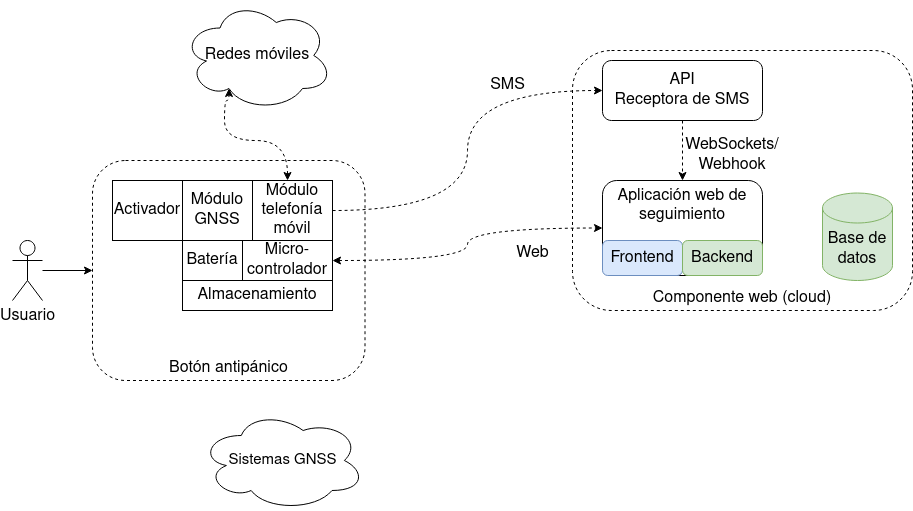
\includegraphics[width=.9\textwidth]{./Figures/diagBloques.png}
	\caption{Diagrama en bloques del dispositivo y el sistema web}
	\label{fig:texmaker}
\end{figure}

\subsection{Botones antipánico}

Un botón antipánico hace referencia a un dispositivo pequeño y portátil, con una batería, que permite que una persona ante una situación de emergencia, presione el dispositivo para generar una alerta y esta sea recepcionada en un sistema de monitoreo.

Estos dispositivos generalmente son brindados por las autoridades, o también pueden ser brindados por empresas de seguridad privadas. Sus beneficiarios suelen ser:
\begin{itemize}
\item Personas en situación de violencia de género.	
\item Personas en situación de violencia intrafamiliar.
\item Establecimientos donde pueden ocurrir situaciones de violencia y es necesario dar rápidamente aviso a las autoridades.
\item Agente o sereno cuyo recorrido debe ser registrado.
\item Entre otros.
\end{itemize}

Entre sus funcionalidades, suelen poseer:
\begin{itemize}
\item Conectividad a la red de telefonía móvil (\textit{Global System for Mobile communications} o GSM).
\item Acceso a datos móviles (\textit{General Packet Radio Service} o GPRS).
\item Conectividad a sistemas de geoposicionamiento satelital (\textit{Global Navigation Satellite System} o GNSS).
\item Botón de disparo de alerta.
\item Reporte periódico de ubicación por mensaje de texto (SMS) o vía web.
\end{itemize}

Un detalle interesante respecto a estos dispositivos es que generalmente se comercializan en dos formatos:

\begin{itemize}
\item Dispositivo personal: dispositivo embebido que puede ser llevado como colgante, en la muñeca o en el bolsillo. Tiene una autonomía limitada.
\item Dispositivo para móviles: también conocido como AVL o \textit{Automatic Vehicle Location}; además de contar con antenas externas para mayor precisión, cuenta con cables para conexión a la batería de los vehículos, permitiendo tener una mayor autonomía.
\end{itemize}


En relación a este trabajo, se planteó el desarrollo del prototipo de un botón geolocalizador y una plataforma web a modo de prueba de concepto, para la recepción de alertas.

%----------------------------------------------------------------------------------------

\section{Motivación}

El autor del trabajo ha trabajado anteriormente con este tipo de soluciones, principalmente en la adquisición, configuración, implementación y soporte de botones antipánico disponibles en el mercado. Se detectó y se llegó a la conclusión, respecto a los dispositivos, de que estos presentan los siguientes inconvenientes:

\begin{itemize}
\item Especificaciones de hardware obsoletas.
\item Documentación escasa, desactualizada o incluso incorrecta en algunos casos.
\item Poca fiabilidad de dispositivo (dificultad para configurarlos, mala señal en ambientes \textit{indoor}, desconfianza al momento de utilizarlo).
\item Inconsistencias entre dispositivos idénticos.
\item Poca duración de batería (desde aproximadamente 24 horas hasta 3 o 4 días como máximo, cuando lo deseable para el beneficiario final del botón es de al menos 5 o 6 días).
\item Precio exageradamente elevado y muchas dificultades para adquirirlos mediante proveedores, más en períodos de alta inflación.
\item Nulas características de seguridad.
\end{itemize}

Se investigaron y revisaron diferentes alternativas en el mercado, así como también se trabajó con dispositivos utilizados por sistemas de la competencia, llegando a conclusiones similares: no se encuentran dispositivos aceptables cuyo costo sea accesible.

Todas estas cuestiones nombradas anteriormente son las que motivaron la formulación del proyecto, siendo necesario disponer de mínimamente un dispositivo embebido con un conjunto de funcionalidades definidas, y un sistema web que permita recepcionar la información del botón.

Otras motivaciones menores del trabajo, pero igualmente muy relacionadas a la especialización, fueron:
\begin{itemize}
\item Profundizar en el uso de frameworks para \textit{Single Web Applications} o SPAs.
\item Poder aplicar los conocimientos trabajados en relación a tecnologías \textit{cloud} y desarrollo de APIs web.
\end{itemize}

%----------------------------------------------------------------------------------------

\section{Objetivos y alcance}

En relación a los objetivos de alto nivel del trabajo, estos fueron:
\begin{itemize}
\item Investigación y determinación de un conjunto de módulos de hardware que sean adecuados para la construcción del prototipo.
\item Diseño y construcción un prototipo de botón antipánico que permita validar las decisiones tecnológicas.
\item Tener fiabilidad superior sobre ciertas características, en comparación con algunos de los dispositivos disponibles en el mercado.
\item Desarrollo de un sistema web a modo de prueba de concepto para el uso del dispositivo.
\end{itemize}

Respecto a los objetivos por componente, estos fueron:

\begin{table}[h]
	\centering
	\caption[Resumen de objetivos]{Resumen de objetivos del trabajo}
	\begin{tabular}{l c c}    
		\toprule
		\textbf{Componente} 	 & \textbf{Objetivo} 	  \\
		\midrule
		Prototipo & Duración de la batería 				\\		
		Prototipo & Calidad de señal de GSM en ambientes cerrados y abiertos			\\
		Prototipo & Calidad de señal de GNSS en ambientes cerrados y abiertos			\\
		Prototipo & Tiempo de actualización de la ubicación (\textit{time-to-first-fix}) \\
		Prototipo & Envío de alertas mediante pulsador		\\
		Sistema web & Recepción de SMS de alertas			\\
		Sistema web & Alta de dispositivos			\\
		Sistema web & Visualización de alertas en tiempo real			\\
		Sistema web & Despliegue en un entorno \textit{cloud}			\\
		\bottomrule
		\hline
	\end{tabular}
	\label{tab:peces}
\end{table}

No se incluyeron dentro del alcance del trabajo, las siguientes características:

\begin{itemize}
\item Aplicación web productiva para gestionar las activaciones del botón antipánico. Por productiva se refiere a que pueda ser ofrecida al mercado o utilizable por usuarios encargados del monitoreo.
\item Desarrollo de un dispositivo listo para reemplazar dispositivos existentes, es decir que no sea un prototipo.
\item Desarrollo de un contenedor físico para el dispositivo.
\end{itemize}

Además, durante el desarrollo del trabajo, se fueron detectando diferentes cuestiones técnicas a resolver, que modificaron algunos objetivos planteados inicialmente.

%----------------------------------------------------------------------------------------

\section{Soluciones comerciales similares}

Retomando los inconvenientes de soluciones actuales, se presentan a continuación algunos modelos conocidos y utilizados en el mercado local. Estos dos modelos sufren los inconvenientes nombrados en las secciones anteriores: el motivo de fondo es que existen muchos clones de estos modelos, resultando muy difícil determinar si se está trabajando con un dispositivo original o un clon con posibles problemas \citep{CLONES:1}.
\subsection{LK109}

LK109 es el nombre de un dispositivo geolocalizador que trabaja con redes GSM y GPRS, y usa \textit{Global Positioning System} (GPS) como sistema de GNSS. Existe también una versión que trabaja con redes 3G, cuyo costo es superior. Entre sus características más interesantes se encuentran \citep{LK109MANUAL:1}:
\begin{itemize}
\item Indicadores de estado: batería, señal de GPS y señal de GSM.
\item Posibilidad de reportar la ubicación mediante TCP o SMS.
\item Reporte de ubicación en tiempo real, con una perioricidad configurable.
\item Posibilidad de monitorear de forma remota el entorno del dispositivo mediante un parlante.
\item Autonomía de 240 horas o 10 días.
\end{itemize}

\begin{figure}[H]
	\centering
	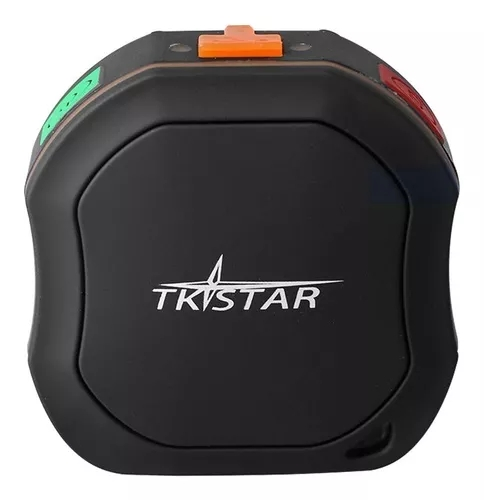
\includegraphics[width=.6\textwidth]{./Figures/lk109.jpg}
	\caption{Imagen del botón LK109}
	\label{fig:texmaker}
\end{figure}

\subsection{TK102B}

TK102B es el nombre de otro dispositivo geolocalizador que trabaja con redes GSM y GPRS, y usa \textit{Global Positioning System} (GPS) como sistema de GNSS. Entre sus características más relevantes se encuentran \citep{TK102BMANUAL:1}:
\begin{itemize}
\item Indicadores de estado: batería, señal de GPS y señal de GSM.
\item Posibilidad de reportar la ubicación mediante TCP o SMS, incluyendo la dirección aproximada, mediante geodecodificación inversa.
\item Reporte de ubicación en tiempo real, con una periodicidad configurable.
\item Posibilidad de monitorear de forma remota el entorno del dispositivo mediante un parlante.
\item Autonomía de 80 horas o 3 días aproximadamente.
\end{itemize}

\begin{figure}[H]
	\centering
	
\includegraphics[width=.6\textwidth]{./Figures/tk102b.jpg}
	\caption{Imagen del botón TK102B}
	\label{fig:texmaker}
\end{figure}

\begin{table}[h]
	\centering
	\caption[Tabla comparativa]{Tabla comparativa de los dos modelos}
	\begin{tabular}{l c c}    
		\toprule
		\textbf{Característica} 	 & \textbf{LK109} & \textbf{TK102B}	  \\
		\midrule
		Conectividad & GSM, GPRS, SMS & 	GSM, GPRS, SMS			\\		
		Reporte periódico & Si & Si			\\
		Autonomía (horas) & 240 & 80		\\
		Indicadores de estado & Si & Si \\
		Escucha remota & Si & Si \\
		Protocolo de comunicación & h02 & gps103 \\
		\bottomrule
		\hline
	\end{tabular}
	\label{tab:peces}
\end{table}

Respecto al ítem de autonomía, no se ha podido comprobar en la práctica que la duración sea la indicada (siempre es mucho menor, entre 12 y 24 horas), a excepción del uso mediante \textit{sleep} o ahorro de batería, que no tiene utilidad para las aplicaciones de seguimiento de una persona. Esto es debido a que en el modo de ahorro de batería, la ubicación se actualiza posterior al envío de una alerta y no antes, resultando ínutil la ubicación reportada.

En relación al ítem de escucha remota, es decir la posibilidad de escuchar lo que ocurre alrededor del dispositivo, no se ha podido verificar para varios dispositivos; de todas maneras no resulta, al menos para los casos de uso reales, una funcionalidad atractiva. Las funcionalidades que se deben cumplir y validar a rajatabla son:
\begin{itemize}
	\item Precisión al momento de obtener la ubicación.
	\item Autonomía considerable de la batería.
	\item Rapidez para obtener señal de GSM y GNSS.
\end{itemize}

Por este motivo, es que no se intentó entre los objetivos iniciales ir más allá de las características iniciales.

\section{Personalizando la plantilla, el archivo \file{memoria.tex}}
\label{sec:FillingFile}

Para personalizar la plantilla se debe incorporar la información propia en los distintos archivos \file{.tex}. 

Primero abrir \file{memoria.tex} con TexMaker (o el editor de su preferencia). Se debe ubicar dentro del archivo el bloque de código titulado \emph{INFORMACIÓN DE LA PORTADA} donde se deben incorporar los primeros datos personales con los que se construirá automáticamente la portada.


%----------------------------------------------------------------------------------------

\section{El código del archivo \file{memoria.tex} explicado}

El archivo \file{memoria.tex} contiene la estructura del documento y es el archivo de mayor jerarquía de la memoria.  Podría ser equiparable a la función \emph{main()} de un programa en C, o mejor dicho al archivo fuente .c donde se encuentra definida la función main().

La estructura básica de cualquier documento de \LaTeX{} comienza con la definición de clase del documento, es seguida por un preámbulo donde se pueden agregar funcionalidades con el uso de \texttt{paquetes} (equiparables a bibliotecas de C), y finalmente, termina con el cuerpo del documento, donde irá el contenido de la memoria.

\lstset{%
  basicstyle=\small\ttfamily,
  language=[LaTeX]{TeX}
}

\begin{lstlisting}
\documentclass{article}  <- Definicion de clase
\usepackage{listings}	 <- Preambulo

\begin{document}	 <- Comienzo del contenido propio 
	Hello world!
\end{document}
\end{lstlisting}


El archivo \file{memoria.tex} se encuentra densamente comentado para explicar qué páginas, secciones y elementos de formato está creando el código \LaTeX{} en cada línea. El código está dividido en bloques con nombres en mayúsculas para que resulte evidente qué es lo que hace esa porción de código en particular. Inicialmente puede parecer que hay mucho código \LaTeX{}, pero es principalmente código para dar formato a la memoria por lo que no requiere intervención del usuario de la plantilla.  Sí se deben personalizar con su información los bloques indicados como:

\begin{itemize}
	\item Informacion de la memoria
	\item Resumen
	\item Agradecimientos
	\item Dedicatoria
\end{itemize}

El índice de contenidos, las listas de figura de tablas se generan en forma automática y no requieren intervención ni edición manual por parte del usuario de la plantilla. 

En la parte final del documento se encuentran los capítulos y los apéndices.  Por defecto se incluyen los 5 capítulos propuestos que se encuentran en la carpeta /Chapters. Cada capítulo se debe escribir en un archivo .tex separado y se debe poner en la carpeta \emph{Chapters} con el nombre \file{Chapter1}, \file{Chapter2}, etc\ldots El código para incluir capítulos desde archivos externos se muestra a continuación.

\begin{verbatim}
	% Chapter 1

\chapter{Introducción general} % Main chapter title

\label{Chapter1} % For referencing the chapter elsewhere, use \ref{Chapter1} 
\label{IntroGeneral}

%----------------------------------------------------------------------------------------

% Define some commands to keep the formatting separated from the content 
\newcommand{\keyword}[1]{\textbf{#1}}
\newcommand{\tabhead}[1]{\textbf{#1}}
\newcommand{\code}[1]{\texttt{#1}}
\newcommand{\file}[1]{\texttt{\bfseries#1}}
\newcommand{\option}[1]{\texttt{\itshape#1}}
\newcommand{\grados}{$^{\circ}$}

%----------------------------------------------------------------------------------------

%\section{Introducción}

Este capítulo presenta una introducción a los conceptos básicos de la temática del trabajo y explica las principales causas que motivaron el desarrollo del proyecto, junto con los objetivos que se buscaron alcanzar.

%----------------------------------------------------------------------------------------
\section{Planteo básico}

Existen en la actualidad diferentes soluciones en lo que respecta a la prevención o seguridad ciudadana \citep{PNUD:1}. Estos sistemas centralizan información en tiempo real de cámaras de seguridad, móviles de las fuerzas de seguridad, entre otros. Además, suelen incorporar alguna funcionalidad para que un ciudadano, ante una situación de emergencia, pueda dar aviso a las autoridades. El mecanismo para notificar puede ser una aplicación móvil, un dispositivo geolocalizador u otra alternativa pero el objetivo es el mismo.

\begin{figure}[htbp]
	\centering
	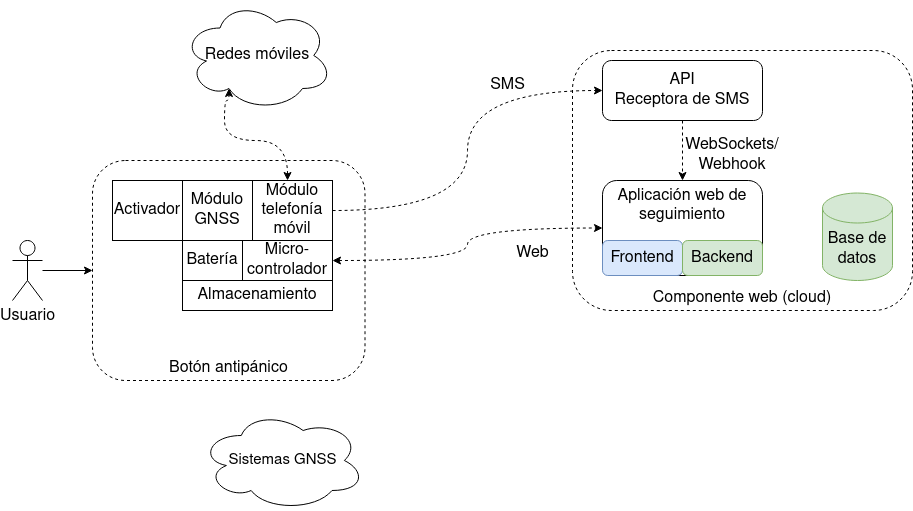
\includegraphics[width=.9\textwidth]{./Figures/diagBloques.png}
	\caption{Diagrama en bloques del dispositivo y el sistema web}
	\label{fig:texmaker}
\end{figure}

\subsection{Botones antipánico}

Un botón antipánico hace referencia a un dispositivo pequeño y portátil, con una batería, que permite que una persona ante una situación de emergencia, presione el dispositivo para generar una alerta y esta sea recepcionada en un sistema de monitoreo.

Estos dispositivos generalmente son brindados por las autoridades, o también pueden ser brindados por empresas de seguridad privadas. Sus beneficiarios suelen ser:
\begin{itemize}
\item Personas en situación de violencia de género.	
\item Personas en situación de violencia intrafamiliar.
\item Establecimientos donde pueden ocurrir situaciones de violencia y es necesario dar rápidamente aviso a las autoridades.
\item Agente o sereno cuyo recorrido debe ser registrado.
\item Entre otros.
\end{itemize}

Entre sus funcionalidades, suelen poseer:
\begin{itemize}
\item Conectividad a la red de telefonía móvil (\textit{Global System for Mobile communications} o GSM).
\item Acceso a datos móviles (\textit{General Packet Radio Service} o GPRS).
\item Conectividad a sistemas de geoposicionamiento satelital (\textit{Global Navigation Satellite System} o GNSS).
\item Botón de disparo de alerta.
\item Reporte periódico de ubicación por mensaje de texto (SMS) o vía web.
\end{itemize}

Un detalle interesante respecto a estos dispositivos es que generalmente se comercializan en dos formatos:

\begin{itemize}
\item Dispositivo personal: dispositivo embebido que puede ser llevado como colgante, en la muñeca o en el bolsillo. Tiene una autonomía limitada.
\item Dispositivo para móviles: también conocido como AVL o \textit{Automatic Vehicle Location}; además de contar con antenas externas para mayor precisión, cuenta con cables para conexión a la batería de los vehículos, permitiendo tener una mayor autonomía.
\end{itemize}


En relación a este trabajo, se planteó el desarrollo del prototipo de un botón geolocalizador y una plataforma web a modo de prueba de concepto, para la recepción de alertas.

%----------------------------------------------------------------------------------------

\section{Motivación}

El autor del trabajo ha trabajado anteriormente con este tipo de soluciones, principalmente en la adquisición, configuración, implementación y soporte de botones antipánico disponibles en el mercado. Se detectó y se llegó a la conclusión, respecto a los dispositivos, de que estos presentan los siguientes inconvenientes:

\begin{itemize}
\item Especificaciones de hardware obsoletas.
\item Documentación escasa, desactualizada o incluso incorrecta en algunos casos.
\item Poca fiabilidad de dispositivo (dificultad para configurarlos, mala señal en ambientes \textit{indoor}, desconfianza al momento de utilizarlo).
\item Inconsistencias entre dispositivos idénticos.
\item Poca duración de batería (desde aproximadamente 24 horas hasta 3 o 4 días como máximo, cuando lo deseable para el beneficiario final del botón es de al menos 5 o 6 días).
\item Precio exageradamente elevado y muchas dificultades para adquirirlos mediante proveedores, más en períodos de alta inflación.
\item Nulas características de seguridad.
\end{itemize}

Se investigaron y revisaron diferentes alternativas en el mercado, así como también se trabajó con dispositivos utilizados por sistemas de la competencia, llegando a conclusiones similares: no se encuentran dispositivos aceptables cuyo costo sea accesible.

Todas estas cuestiones nombradas anteriormente son las que motivaron la formulación del proyecto, siendo necesario disponer de mínimamente un dispositivo embebido con un conjunto de funcionalidades definidas, y un sistema web que permita recepcionar la información del botón.

Otras motivaciones menores del trabajo, pero igualmente muy relacionadas a la especialización, fueron:
\begin{itemize}
\item Profundizar en el uso de frameworks para \textit{Single Web Applications} o SPAs.
\item Poder aplicar los conocimientos trabajados en relación a tecnologías \textit{cloud} y desarrollo de APIs web.
\end{itemize}

%----------------------------------------------------------------------------------------

\section{Objetivos y alcance}

En relación a los objetivos de alto nivel del trabajo, estos fueron:
\begin{itemize}
\item Investigación y determinación de un conjunto de módulos de hardware que sean adecuados para la construcción del prototipo.
\item Diseño y construcción un prototipo de botón antipánico que permita validar las decisiones tecnológicas.
\item Tener fiabilidad superior sobre ciertas características, en comparación con algunos de los dispositivos disponibles en el mercado.
\item Desarrollo de un sistema web a modo de prueba de concepto para el uso del dispositivo.
\end{itemize}

Respecto a los objetivos por componente, estos fueron:

\begin{table}[h]
	\centering
	\caption[Resumen de objetivos]{Resumen de objetivos del trabajo}
	\begin{tabular}{l c c}    
		\toprule
		\textbf{Componente} 	 & \textbf{Objetivo} 	  \\
		\midrule
		Prototipo & Duración de la batería 				\\		
		Prototipo & Calidad de señal de GSM en ambientes cerrados y abiertos			\\
		Prototipo & Calidad de señal de GNSS en ambientes cerrados y abiertos			\\
		Prototipo & Tiempo de actualización de la ubicación (\textit{time-to-first-fix}) \\
		Prototipo & Envío de alertas mediante pulsador		\\
		Sistema web & Recepción de SMS de alertas			\\
		Sistema web & Alta de dispositivos			\\
		Sistema web & Visualización de alertas en tiempo real			\\
		Sistema web & Despliegue en un entorno \textit{cloud}			\\
		\bottomrule
		\hline
	\end{tabular}
	\label{tab:peces}
\end{table}

No se incluyeron dentro del alcance del trabajo, las siguientes características:

\begin{itemize}
\item Aplicación web productiva para gestionar las activaciones del botón antipánico. Por productiva se refiere a que pueda ser ofrecida al mercado o utilizable por usuarios encargados del monitoreo.
\item Desarrollo de un dispositivo listo para reemplazar dispositivos existentes, es decir que no sea un prototipo.
\item Desarrollo de un contenedor físico para el dispositivo.
\end{itemize}

Además, durante el desarrollo del trabajo, se fueron detectando diferentes cuestiones técnicas a resolver, que modificaron algunos objetivos planteados inicialmente.

%----------------------------------------------------------------------------------------

\section{Soluciones comerciales similares}

Retomando los inconvenientes de soluciones actuales, se presentan a continuación algunos modelos conocidos y utilizados en el mercado local. Estos dos modelos sufren los inconvenientes nombrados en las secciones anteriores: el motivo de fondo es que existen muchos clones de estos modelos, resultando muy difícil determinar si se está trabajando con un dispositivo original o un clon con posibles problemas \citep{CLONES:1}.
\subsection{LK109}

LK109 es el nombre de un dispositivo geolocalizador que trabaja con redes GSM y GPRS, y usa \textit{Global Positioning System} (GPS) como sistema de GNSS. Existe también una versión que trabaja con redes 3G, cuyo costo es superior. Entre sus características más interesantes se encuentran \citep{LK109MANUAL:1}:
\begin{itemize}
\item Indicadores de estado: batería, señal de GPS y señal de GSM.
\item Posibilidad de reportar la ubicación mediante TCP o SMS.
\item Reporte de ubicación en tiempo real, con una perioricidad configurable.
\item Posibilidad de monitorear de forma remota el entorno del dispositivo mediante un parlante.
\item Autonomía de 240 horas o 10 días.
\end{itemize}

\begin{figure}[H]
	\centering
	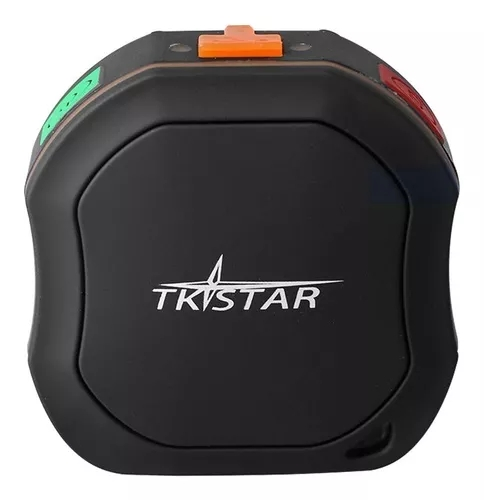
\includegraphics[width=.6\textwidth]{./Figures/lk109.jpg}
	\caption{Imagen del botón LK109}
	\label{fig:texmaker}
\end{figure}

\subsection{TK102B}

TK102B es el nombre de otro dispositivo geolocalizador que trabaja con redes GSM y GPRS, y usa \textit{Global Positioning System} (GPS) como sistema de GNSS. Entre sus características más relevantes se encuentran \citep{TK102BMANUAL:1}:
\begin{itemize}
\item Indicadores de estado: batería, señal de GPS y señal de GSM.
\item Posibilidad de reportar la ubicación mediante TCP o SMS, incluyendo la dirección aproximada, mediante geodecodificación inversa.
\item Reporte de ubicación en tiempo real, con una periodicidad configurable.
\item Posibilidad de monitorear de forma remota el entorno del dispositivo mediante un parlante.
\item Autonomía de 80 horas o 3 días aproximadamente.
\end{itemize}

\begin{figure}[H]
	\centering
	
\includegraphics[width=.6\textwidth]{./Figures/tk102b.jpg}
	\caption{Imagen del botón TK102B}
	\label{fig:texmaker}
\end{figure}

\begin{table}[h]
	\centering
	\caption[Tabla comparativa]{Tabla comparativa de los dos modelos}
	\begin{tabular}{l c c}    
		\toprule
		\textbf{Característica} 	 & \textbf{LK109} & \textbf{TK102B}	  \\
		\midrule
		Conectividad & GSM, GPRS, SMS & 	GSM, GPRS, SMS			\\		
		Reporte periódico & Si & Si			\\
		Autonomía (horas) & 240 & 80		\\
		Indicadores de estado & Si & Si \\
		Escucha remota & Si & Si \\
		Protocolo de comunicación & h02 & gps103 \\
		\bottomrule
		\hline
	\end{tabular}
	\label{tab:peces}
\end{table}

Respecto al ítem de autonomía, no se ha podido comprobar en la práctica que la duración sea la indicada (siempre es mucho menor, entre 12 y 24 horas), a excepción del uso mediante \textit{sleep} o ahorro de batería, que no tiene utilidad para las aplicaciones de seguimiento de una persona. Esto es debido a que en el modo de ahorro de batería, la ubicación se actualiza posterior al envío de una alerta y no antes, resultando ínutil la ubicación reportada.

En relación al ítem de escucha remota, es decir la posibilidad de escuchar lo que ocurre alrededor del dispositivo, no se ha podido verificar para varios dispositivos; de todas maneras no resulta, al menos para los casos de uso reales, una funcionalidad atractiva. Las funcionalidades que se deben cumplir y validar a rajatabla son:
\begin{itemize}
	\item Precisión al momento de obtener la ubicación.
	\item Autonomía considerable de la batería.
	\item Rapidez para obtener señal de GSM y GNSS.
\end{itemize}

Por este motivo, es que no se intentó entre los objetivos iniciales ir más allá de las características iniciales.
	\chapter{Introducción específica} % Main chapter title

\label{Chapter2}
%----------------------------------------------------------------------------------------
%	SECTION 1
%----------------------------------------------------------------------------------------
En este capítulo se hace una presentación de cuestiones técnicas particulares del trabajo, una descripción de alto nivel de las tecnologías involucradas y las herramientas y servicios externos que formaron parte del desarrollo, así como también los componentes de hardware empleados.

\section{Particularidades de los sistemas de botones antipánico}

Es necesario, en primer lugar, hacer una introducción a las características que deben tener las soluciones de este tipo, junto con sus limitaciones y particularidades técnicas. Cualquier desarrollo de este tipo debe considerar las siguientes características para los módulos de hardware y software.

\subsection{Características del hardware}

Los botones antipánico y dispositivos geolocalizadores suelen ser utilizados en zonas donde la cobertura de telefonía móvil es muy baja. Es decir, se cuenta con conectividad limitada para llamadas y mensajes, y prácticamente no hay cobertura para datos móviles o es de baja tasa de transferencia. La tecnología más presente es la de GPRS o 2G\citep{NPERF:1}, ya que es la red de mayor alcance, pero también la de menor ancho de banda.
Esto impone una restricción respecto a la conectividad, por lo que la mayoría de los dispositivos tienen las siguientes características respecto al método de comunicación:
\begin{itemize}
	\item Comunicación vía SMS, TCP o UDP para configuración y envío de datos.
	\item Comunicación vía protocolos personalizados\citep{PROTOCOLS:1} para reducir el \textit{overhead} de datos.
	\item Mecanismos para almacenar datos en caso de perder conectividad.
\end{itemize}

Debido a que, dentro del alcance del trabajo se apunta a configuración y envío de mensajes de alerta, se consideró innecesario, para estas funciones, requerir otro medio adicional. No se considera apropiado usar un método de comunicación que pueda no ser fiable, como lo son los datos móviles en zonas donde la conectividad es baja.

Por otra parte, otro punto importante respecto a estos dispositivos, es su capacidad de obtener señal aceptable tanto de GSM como GNSS en ambientes \textit{indoor} y \textit{outdoor}. Prácticamente todos los botones antipánico poseen antenas internas y sin alimentación activa, por lo que su capacidad para adquirir un nivel de señal aceptable es limitada; esto introduce varios puntos a favor y en contra:
\begin{itemize}
	\item No generan un consumo de energía adicional.
	\item Su tiempo de \textit{startup}, es decir, hasta que adquieren un nivel de señal operativo aceptable, es elevado si están en ambientes cerrados.
	\item Su precisión suele ser baja en ambientes cerrados, lo cual puede ser un problema en situaciones de emergencia.
	\item El tiempo de actualización de la posición de la persona puede ser elevado si la antena no logra captar una buena señal.
\end{itemize}

\subsection{Características de los sistemas web}

Un sistema web, al requerir estar en comunicación con un dispositivo y mostrar su información en tiempo real, debe contar, idealmente, con las siguientes características:
\begin{itemize}
	\item No requerir ningún software adicional para su acceso y uso más allá de un navegador web y conexión a Internet.
	\item Poder recibir mensajes de texto, es decir, tener un número telefónico virtual asociado.
	\item Enviar actualizaciones \textit{push} al navegador del usuario en tiempo real.
\end{itemize}

Se presentan algunos desafíos respecto al segundo y tercer punto. Para la recepción de SMS, es necesario tener integrada una central de telefonía virtual o implementar un \textit{Short Message Service Center} o SMSC, un servicio específico para el ruteo de mensajes de texto desde y hacia la web. Respecto al tercer punto, resulta obligatoria la implementación de algún mecanismo de actualización en tiempo real desde el servidor hacia el cliente, el navegador web, y no al revés, como puede ser \textit{WebSocket}.

En algunos casos, también debería permitir comunicación bidireccional con los dispositivos, para que un operador pueda configurarlos \textit{on-demand}. De todas maneras, debido a que está fuera del alcance del trabajo, no se planteó el desarrollo de esta característica.

\section{Componentes de hardware utilizados}

\subsection{Microcontrolador ESP32}



Se utilizó un SoC (\textit{System on a Chip}) de la familia ESP32 de Espressif debido a que resulta una opción ideal para el desarrollo de sistemas embebidos y aplicaciones de Internet de las Cosas. Entre las características que resultaron más atractivas para su elección, se destacan\citep{ESP32:1}:
\begin{itemize}
	\item Bajo costo y disponibilidad en el mercado local.
	\item Prestaciones muy interesantes: Wi-Fi, Bluetooth, modos de ahorro de energía, varios periféricos, entre otros.
	\item Gran soporte de la comunidad y disponibilidad de bibliotecas, junto a su documentación.
	\item Ya utilizado en la carrera de especialización.
\end{itemize}

En la figura 2.1 puede observarse un ESP32-S (variante comercial utilizada).

\begin{figure}[H]
	\centering
	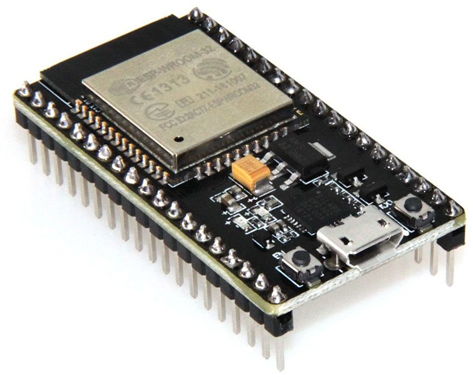
\includegraphics[width=.6\textwidth]{./Figures/esp32s.png}
	\caption{Microcontrolador ESP32-S}
	\label{fig:texmaker}
\end{figure}

Se presentan en la tabla 2.1 algunas alternativas comparadas. De todas maneras, esta comparación no debe ser interpretada linealmente ya que hay placas como Ai Thinker A9G y TTGO T-Call V1.3 que poseen ya módulos integrados, pero todos fueron analizados para el trabajo.

\begin{table}[h]
	\centering
	\caption[Tabla comparativa]{Tabla comparativa de placas de desarrollo}
	\begin{tabular}{l c c c c}    
		\toprule
		\textbf{Característica} 	 & \textbf{ESP32} & \textbf{A9G} & \textbf{LoPy 4} & \textbf{TTGO T-Call}  \\
		\midrule
		Disponibilidad & Baja & No & No & Baja			\\		
		Comunidad & Muy grande & Grande & Poca & Sí			\\
		Costo & Muy bajo & Moderado & Muy elevado & Muy elevado		\\
		Curva aprendizaje & Muy baja & Alta & Baja & Baja \\
		\bottomrule
		\hline
	\end{tabular}
	\label{tab:peces}
\end{table}

\subsection{Módulo GPS NEO-6M}

Para la implementación del módulo de posicionamiento, se decantó por el uso del módulo de GPS NEO-6M desarrollado por la compañía u-blox. Este módulo GPS posee un rango operativo de entre 2.7 V y 3.6 V, siendo muy similar al microcontrolador elegido anteriormente. Tiene modos de ahorro de energía configurables e interfaces de comunicación UART, SPI y I²C\citep{NEO6M:1}. Se analizaron otras alternativas, encontrando mucha similitudes, pero hallando mayor documentación y casos de uso por parte de la comunidad para el NEO-6M. En la figura 2.2 se puede observar una variante de fabricación del NEO-6M.

\begin{figure}[H]
	\centering
	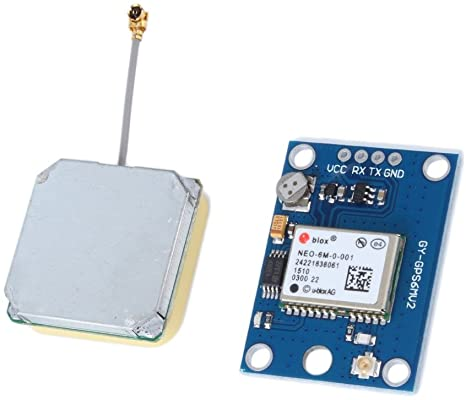
\includegraphics[width=.6\textwidth]{./Figures/neo-6m.jpg}
	\caption{Módulo GPS NEO-6M con una antena externa}
	\label{fig:texmaker}
\end{figure}

Se muestra en la tabla 2.2 una comparativa respecto a otro módulo similar.

\begin{table}[h]
	\centering
	\caption[Tabla comparativa]{Tabla comparativa de placas de desarrollo}
	\begin{tabular}{l c c}    
		\toprule
		\textbf{Característica} 	 & \textbf{Quectel L86} & \textbf{NEO-6M} \\
		\midrule
		Disponibilidad & Moderada & Baja			\\		
		Costo & Moderado & Elevado			\\
		Sistemas GNSS & GPS & GPS, GLONASS, Galileo		\\
		\bottomrule
		\hline
	\end{tabular}
	\label{tab:peces}
\end{table}

\subsection{Módulo GSM SIM800L}

Para el desarrollo de la conectividad a las redes de telefonía móvil se utilizó el módulo SIM800L, un chip fabricado por la compañía Simcom. Funciona con un rango de voltaje entre 3.4 V y 4.4 V, y permite la utilización del módulo mediante comandos AT. Estas instrucciones consisten en cadenas de caracteres cortas utilizadas dentro de la industria desde la década de 1980 hasta el día de hoy para la comunicación con módulos, módems, entre otros dispositivos{\citep{AT:1}}. Posee mecanismos para optimizar el consumo de energía pero tiene picos elevados de consumo durante la trasmisión. Respecto a la compatibilidad de generaciones de tecnologías de telefonía móvil, solo soporta hasta 2G\citep{SIM800L:1}. De todas maneras, para los fines del trabajo, resultó suficiente. En la figura 2.3 se puede visualizar el módulo SIM800L con una antena helicoidal, aunque pueden utilizarse otros tipos de antenas con mayor ganancia de potencia.

\begin{figure}[H]
	\centering
	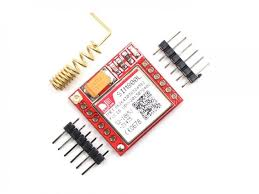
\includegraphics[width=.6\textwidth]{./Figures/sim800l.jpg}
	\caption{Módulo SIM800L}
	\label{fig:texmaker}
\end{figure}

\subsection{Batería 18650 y chip cargador TP4056}



Para la alimentación del microcontrolador y sus módulos, se decidió utilizar una batería recargable del tipo 18650 de Li-ion de 2600 mAh. Este tipo de baterías tiene la ventaja de trabajar con un rango de voltaje apropiado para microcontroladores y módulos, pudiendo además tener una elevada corriente máxima de descarga (hasta 2 A aproximadamente). En la figura 2.4 se puede apreciar el formato de estas, muy similar al de las pilas domésticas. Debido a que requieren un circuito integrado para la alimentación y el control ante sobrecargas, se utilizó un módulo Tp4056 que permite utilizar una entrada micro USB de 5 V, lo cual posibilita, por ejemplo, el uso de un cargador común de teléfono celular. Este circuito se puede visualizar en la figura 2.5.

\begin{figure}[H]
\centering
\begin{minipage}{.5\textwidth}
  \centering
  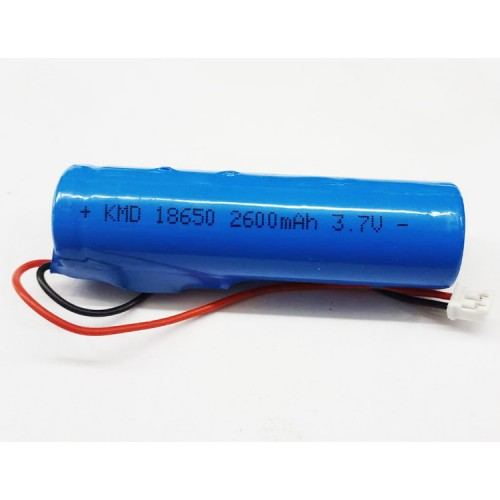
\includegraphics[width=.4\linewidth]{./Figures/18650.jpg}
  \captionof{figure}{Batería 18650}
  \label{fig:test1}
\end{minipage}%
\begin{minipage}{.5\textwidth}
  \centering
  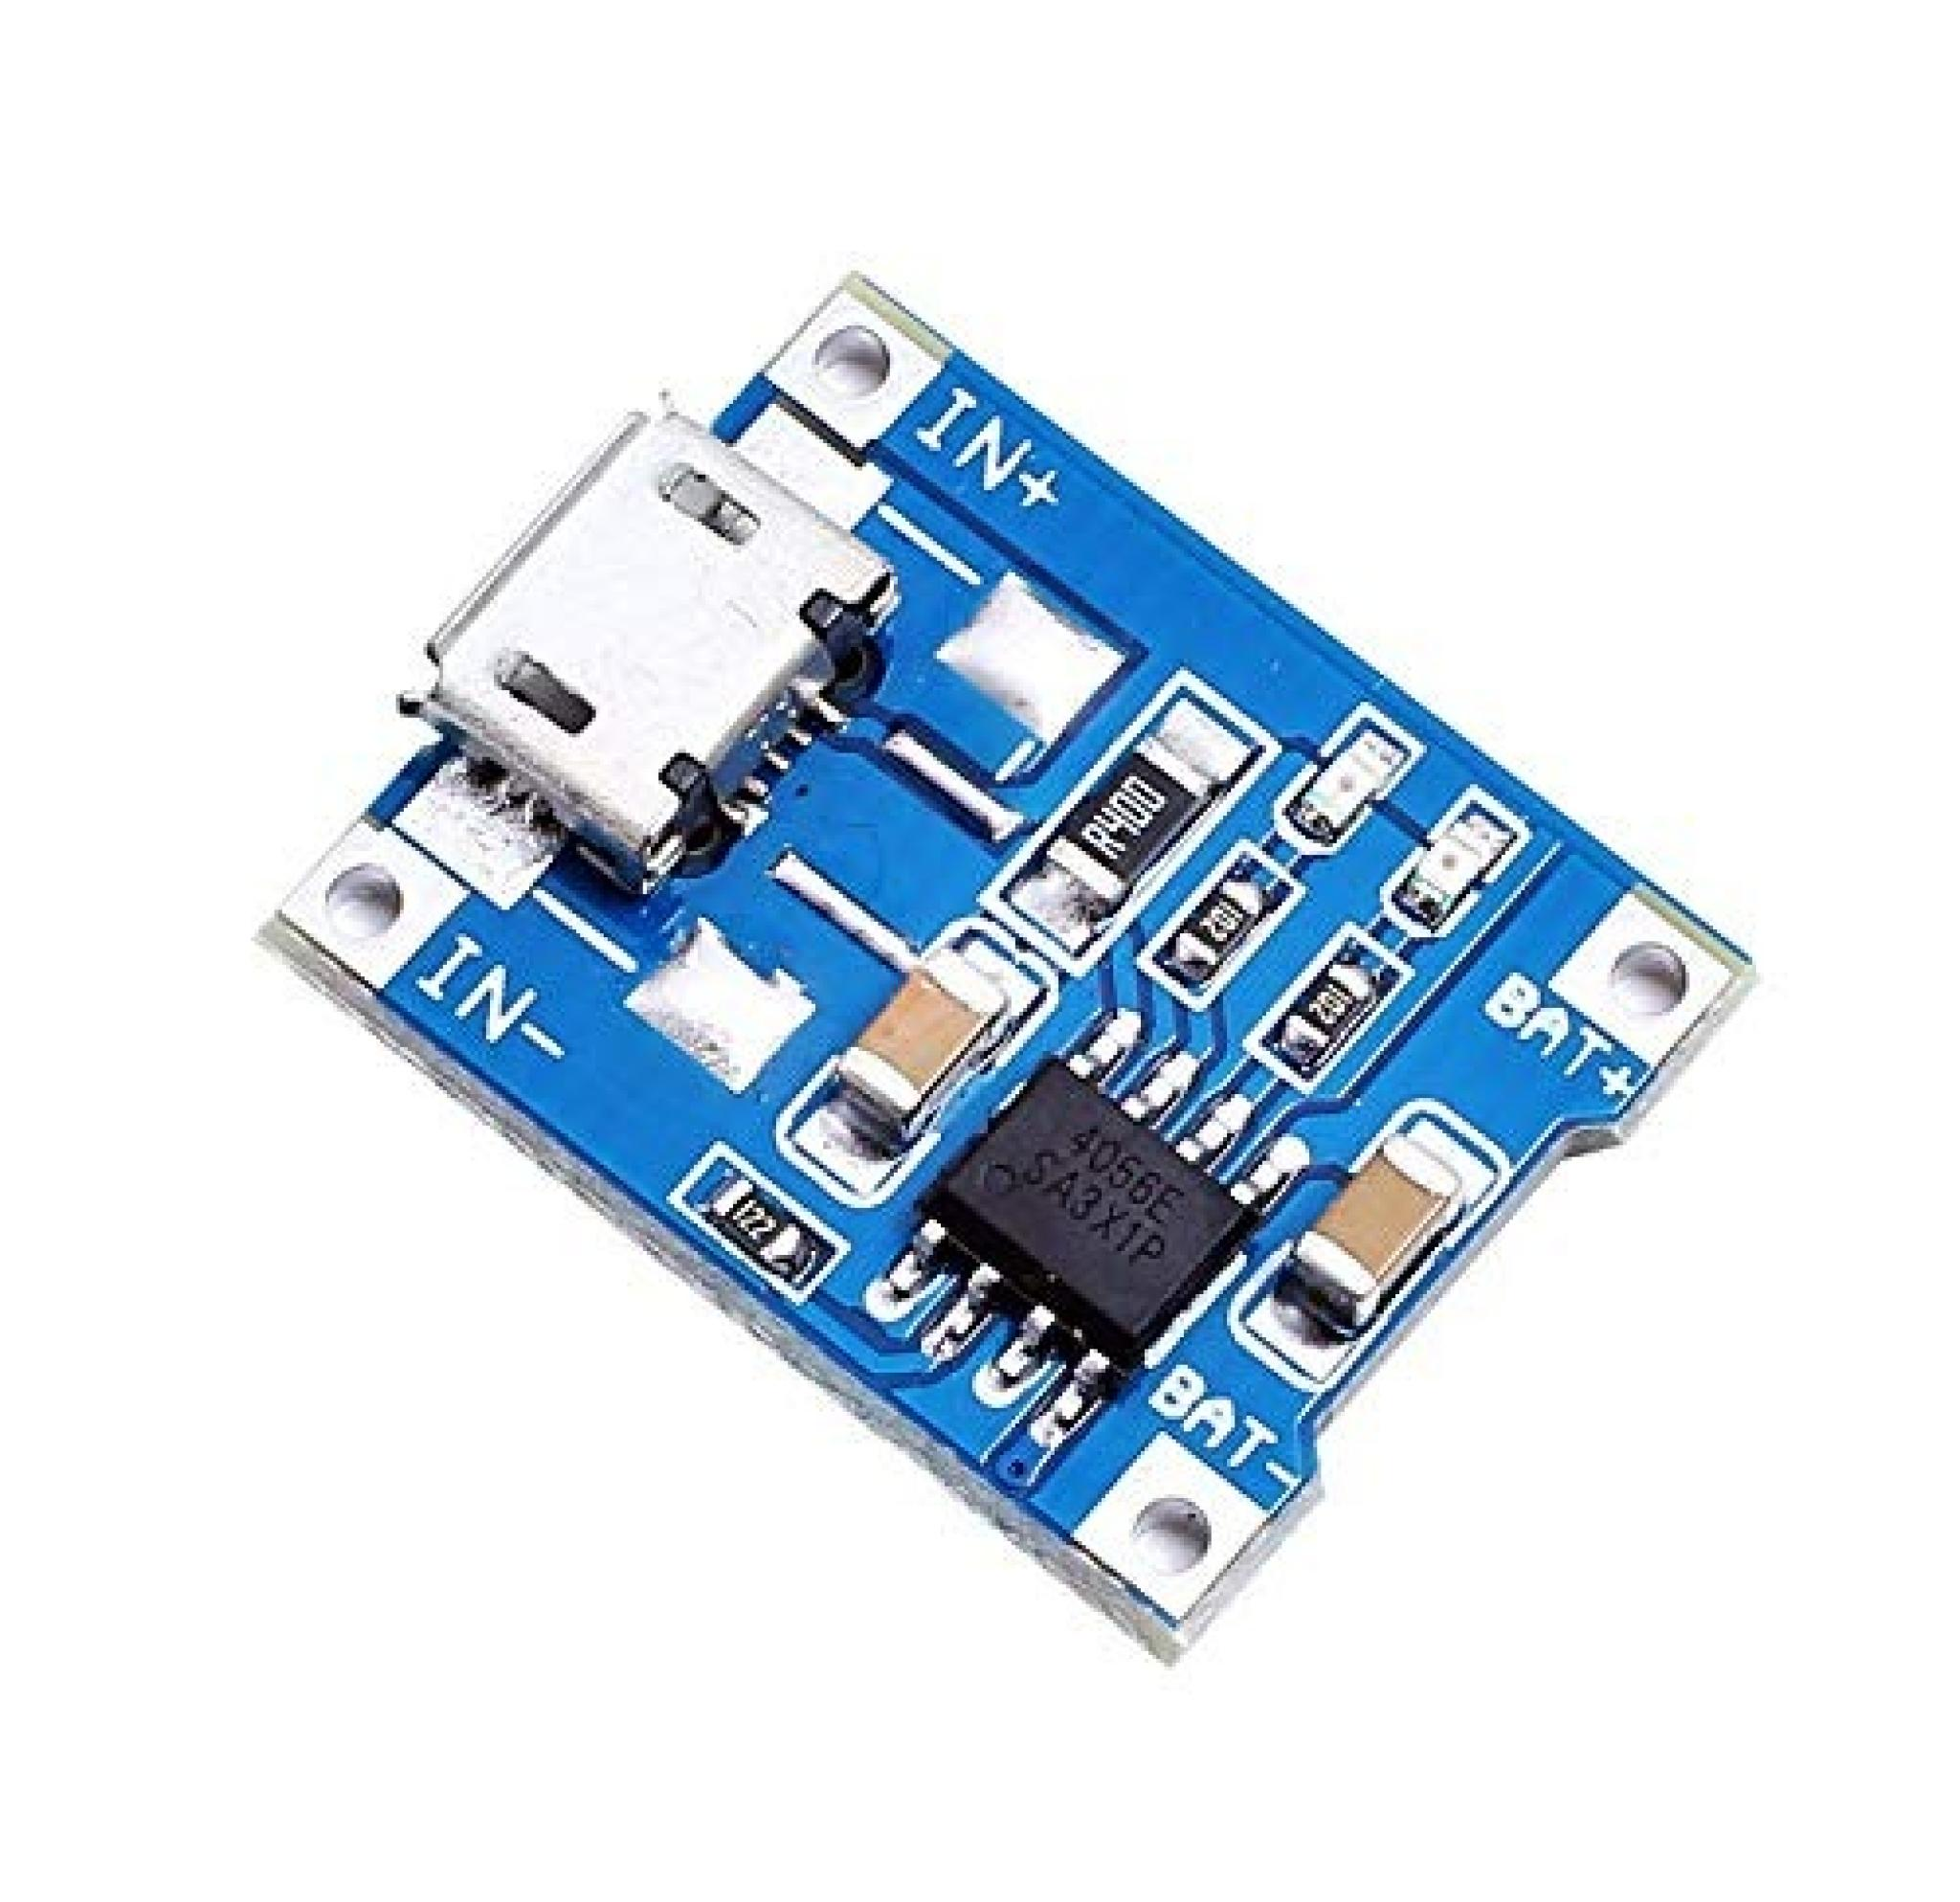
\includegraphics[width=.4\linewidth]{./Figures/tp4056.jpg}
  \captionof{figure}{Circuito Mp4056}
  \label{fig:test2}
\end{minipage}
\end{figure}

\section{Componentes de software utilizados}

\subsection{Django REST framework}

Django REST framework es un conjunto de bibliotecas y herramientas del lenguaje Python para el desarrollo de aplicaciones web y APIs REST. Es el framework \textit{de facto} para el desarrollo web en Python. Entre sus características más interesantes, se encuentran\citep{DJANGO:1}:
\begin{itemize}
	\item Soporte incluído para serialización de datos.
	\item Código modular y reusable mediante \textit{views} y \textit{viewsets}, que son clases de objetos para el armado de interfaces REST sobre el modelo de datos.
	\item Mapeo de bases de datos relacionados a objetos mediante un \textit{Object–relational mapping} (ORM) propio.
	\item Documentación automática para las API por defecto.
	\item Estable desde hace más de una década.
	\item Combina la rapidez para la codificación y flexibilidad de un lenguaje de tipado dinámico junto a un conjunto de características y estructuras para escalar el desarrollo y que siga siendo mantenible.
	\item Soporte para múltiples mecanismos de autenticación ya incluídos.
	\item Bajo uso de recursos.
\end{itemize}

En la tabla 2.3 se puede ver una comparativa con uno de los frameworks web más utilizados de la actualidad\citep{EXPRESS:1}, Express. Se elegió Django para el desarrollo de la API de la aplicación porque se deseó trabajar con un lenguaje como Python, pero con un framework fuertemente estructurado.

\begin{table}[H]
	\centering
	\caption[Tabla comparativa]{Tabla comparativa de frameworks web}
	\begin{tabular}{l c c}    
		\toprule
		\textbf{Característica} 	 & \textbf{Django} & \textbf{Express} \\
		\midrule
		Lenguaje & Python & Javascript \\		
		Curva de aprendizaje & Moderada & Muy baja			\\		
		Arquitectura & Definida & Flexible \\
		Enfoque & Estructurado & Libre/Flexible		\\
		Performance & Muy alta & Extremadamente alta \\
		Baterías incluídas\footnote{El término baterías incluídas se refiere a la disponibilidad por defecto de herramientas y bibliotecas útiles para el desarrollo.} & Sí & No \\
		\bottomrule
		\hline
	\end{tabular}
	\label{tab:peces}
\end{table}

\subsection{Angular}

Angular es un framework de código abierto desarrollado originalmente por Google para la construcción de aplicaciones web del tipo SPA\citep{ANGULAR:1}. Utiliza el lenguaje Typescript que es un \textit{superset} de Javascript, dotándolo de tipado estático y características no presentes en Javascript. Entre sus características más potentes se pueden destacar\citep{ANGULAR:2}:
\begin{itemize}
	\item Framework completo con una estructura definida.
	\item Arquitectura orientada en componentes.
	\item \textit{Binding} de variables bidireccional.
	\item Disponibilidad de muchas bibliotecas y herramientas.
\end{itemize}

Para el desarrollo de las interfaces de usuario, se planteó el uso de \textit{Angular Material}, que es una biblioteca de componentes de interfaces disponible para Angular. Su principal ventaja es la disponibilidad de componentes estándar ya armados y diseño común\citep{ANGULAR:3}.

Para la incorporación de mapas en la aplicación, se definió el uso de Leaftlet, una biblioteca para el desarrollo de mapas en aplicaciones web. Su incorporación a Angular puede hacerse mediante el paquete \textit{ngx-leaftlet}\citep{LEAFLET:1} junto con el proveedor gratuito y \textit{open source} de mapas OpenStreetMap.

\subsection{PostgreSQL}

PostgreSQL es un \textit{relational database management system} o RDBMS de código abierto que hace uso de SQL y es famoso por ser \textit{ACID-compliant}, su gran amplitud de tipos de datos, robustez y extensibilidad\citep{POSTGRES:1}. Es utilizado ampliamente por la industria del software\citep{POSTGRES:2} y se encuentra disponible como una opción por los mayores proveedores de \textit{cloud} de la actualidad. Prácticamente todos los frameworks web permiten conectarse a este motor de bases de datos. 

\subsection{Heroku}

Heroku es un proveedor de infraestructura y servicios en la nube y \textit{Platform as a Service} (PaaS) focalizado en el rápido despliegue y mantenimiento de las aplicaciones web. La principal ventaja de Heroku es que apunta a abstraer al usuario de detalles técnicos y la infraestructura que da soporte a los servicios usados. Se presenta en la tabla 2.4 una comparativa frente a otros proveedores, como Amazon Web Services (AWS) y Google Cloud Platform (GCP).


\begin{table}[H]
	\centering
	\caption[Tabla comparativa]{Tabla comparativa de proveedores \textit{cloud}\citep{CLOUD:1}\citep{CLOUD:2}\citep{CLOUD:3}}
	\begin{tabular}{l c c c}    
		\toprule
		\textbf{Característica} 	 & \textbf{Heroku} & \textbf{AWS} & \textbf{GCP} \\
		\midrule
		Complejidad & Baja & Muy alta & Media-Alta \\		
		Costo & Medio & Bajo & Bajo-Medio			\\		
		Flexibilidad & Baja-Media & Muy alta & Alta \\
		Servicios & Poca oferta & Mucha oferta & Mucha oferta 	\\
		Regiones & Limitadas & Amplias & Amplias \\
		\bottomrule
		\hline
	\end{tabular}
	\label{tab:peces}
\end{table}

\section{Herramientas y servicios de software utilizados}

\subsection{Docker}

Docker es una plataforma \textit{open source} para la contenerización de aplicaciones, con el objetivo de\citep{DOCKER:1}:
\begin{itemize}
	\item Generar versiones de sistemas idénticas entre diferentes ambientes, es decir que un sistema sea portable.
	\item Aislar los recursos del \textit{host} de los sistemas que corren en él.
	\item Reducir los tiempos de despliegue, mantenimiento y soporte de aplicaciones.
\end{itemize}

Docker permite generar imágenes de sistemas siguiendo un conjunto de instrucciones definidas mediante un archivo \textit{Dockerfile}, habilitando generar estas mismas imágenes en otros ambientes.

\subsection{Visual Studio Code}

\textit{Visual Studio Code} es un editor de texto e IDE (Integrated development environment o Entorno de desarrollo integrado) de código abierto desarrollado originalmente por Microsoft\citep{VSCODE:1}. Su flexibilidad y soporte para una cantidad considerable de extensiones para gran parte de los lenguajes y frameworks de la industria lo posicionaron en la última década como uno de los IDE más utilizados.

Permite desarrollar aplicaciones con Python, Javascript/Typescript, incorporando incluso frameworks para el desarrollo de embebidos como es el caso de ESP-IDF\citep{ESPIDF:1} o PlatformIO\citep{PLATFORMIO:1}. La mayoría de proveedores de servicios en la nube han desarrollado extensiones para agilizar el despliegue de aplicaciones en sus servicios.

\subsection{PyGPSClient}

PyGPSClient es una herramienta de escritorio desarrollada en Python para el \textit{debugging} y análisis de varios módulos GNSS de u-blox. Su principal ventaja frente a la herramienta estándar para las pruebas de estos módulos, u-center, es que está disponible para cualquier sistema que soporte Python, en comparación con la anterior que solo se encuentra para Windows\citep{PYGPSCLIENT:1}. En la figura 2.6 es posible observar la aplicación en ejecución, mostrando los mensajes recibidos por el módulo GPS directamente en una terminal y la ubicación geolocalizada del módulo.

\begin{figure}[H]
	\centering
	\includegraphics[width=1\textwidth]{./Figures/pygpsclient.png}
	\caption{Aplicación PyGPSClient}
	\label{fig:texmaker}
\end{figure}

\subsection{Moserial}

Moserial es una aplicación de escritorio orientada al \textit{testing} de dispositivos embebidos, consolas y equipos electrónicos que permiten comunicación vía \textit{Universal Asynchronous Receiver-Transmitter} o UART. Se encuentra disponible para el entorno gráfico GNOME, popular en sistemas GNU/Linux. En la figura 2.7 se muestra su uso, donde se pueden apreciar los datos recibidos vía comunicación serial. Resultó de importancia para la comunicación con el módulo de GSM, SIM800L.

\begin{figure}[H]
	\centering
	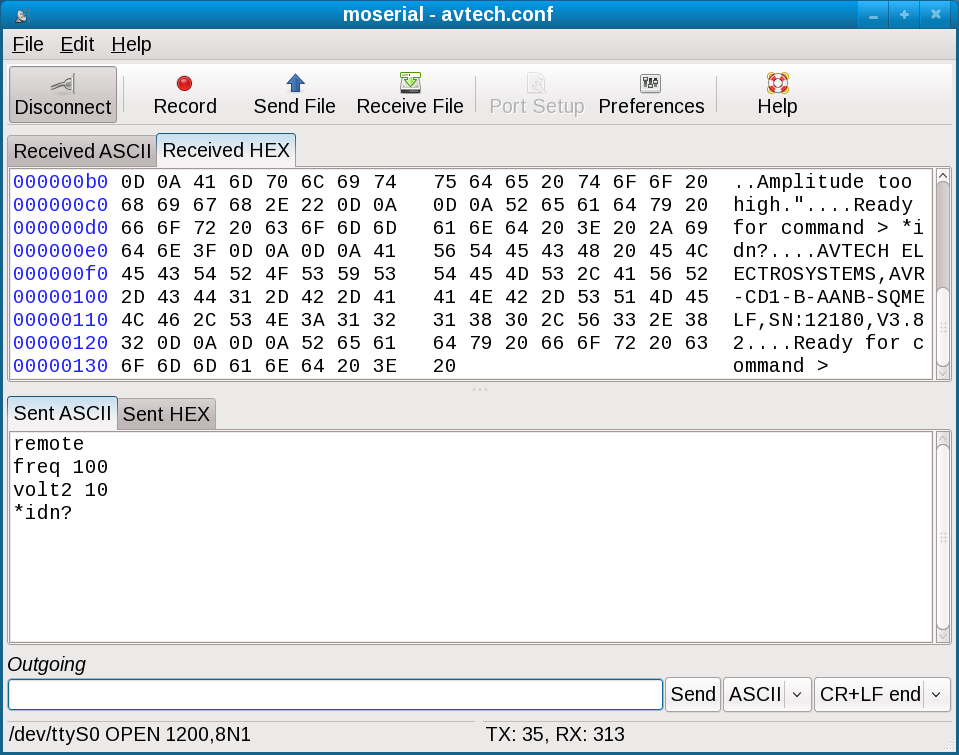
\includegraphics[width=1\textwidth]{./Figures/moserial.png}
	\caption{Aplicación Moserial}
	\label{fig:texmaker}
\end{figure}


\subsection{Twilio}

Twilio es un \textit{Communications Platform as a Service} o CPaSS que ofrece diferentes servicios para el desarrollo de sistemas que requieran funcionalidades relacionadas a telefonía IP\citep{TWILIO:1}. Dentro del trabajo, su principal uso fue para la adquisición de un número de teléfono virtual para la recepción de mensajes de texto provinientes de un dispositivo embebido. Permite acceder a sus servicios mediante varios mecanismos ofrecidos por la plataforma, como APIs web.
 
	\textit{\chapter{Diseño e implementación}} % Main chapter title

\label{Chapter3} % Change X to a consecutive number; for referencing this chapter elsewhere, use \ref{ChapterX}

\definecolor{mygreen}{rgb}{0,0.6,0}
\definecolor{mygray}{rgb}{0.5,0.5,0.5}
\definecolor{mymauve}{rgb}{0.58,0,0.82}

%%%%%%%%%%%%%%%%%%%%%%%%%%%%%%%%%%%%%%%%%%%%%%%%%%%%%%%%%%%%%%%%%%%%%%%%%%%%%
% parámetros para configurar el formato del código en los entornos lstlisting
%%%%%%%%%%%%%%%%%%%%%%%%%%%%%%%%%%%%%%%%%%%%%%%%%%%%%%%%%%%%%%%%%%%%%%%%%%%%%
\lstset{ %
  backgroundcolor=\color{white},   % choose the background color; you must add \usepackage{color} or \usepackage{xcolor}
  basicstyle=\footnotesize,        % the size of the fonts that are used for the code
  breakatwhitespace=false,         % sets if automatic breaks should only happen at whitespace
  breaklines=true,                 % sets automatic line breaking
  captionpos=b,                    % sets the caption-position to bottom
  commentstyle=\color{mygreen},    % comment style
  deletekeywords={...},            % if you want to delete keywords from the given language
  %escapeinside={\%*}{*)},          % if you want to add LaTeX within your code
  %extendedchars=true,              % lets you use non-ASCII characters; for 8-bits encodings only, does not work with UTF-8
  %frame=single,	                % adds a frame around the code
  keepspaces=true,                 % keeps spaces in text, useful for keeping indentation of code (possibly needs columns=flexible)
  keywordstyle=\color{blue},       % keyword style
  language=[ANSI]C,                % the language of the code
  %otherkeywords={*,...},           % if you want to add more keywords to the set
  numbers=left,                    % where to put the line-numbers; possible values are (none, left, right)
  numbersep=5pt,                   % how far the line-numbers are from the code
  numberstyle=\tiny\color{mygray}, % the style that is used for the line-numbers
  rulecolor=\color{black},         % if not set, the frame-color may be changed on line-breaks within not-black text (e.g. comments (green here))
  showspaces=false,                % show spaces everywhere adding particular underscores; it overrides 'showstringspaces'
  showstringspaces=false,          % underline spaces within strings only
  showtabs=false,                  % show tabs within strings adding particular underscores
  stepnumber=1,                    % the step between two line-numbers. If it's 1, each line will be numbered
  stringstyle=\color{mymauve},     % string literal style
  tabsize=2,	                   % sets default tabsize to 2 spaces
  title=\lstname,                  % show the filename of files included with \lstinputlisting; also try caption instead of title
  morecomment=[s]{/*}{*/}
}

En este capítulo se presentan las características de diseño y desarrollo de todos los componentes que forman parte del sistema, presentados en el capítulo 2.

%----------------------------------------------------------------------------------------
%	SECTION 1
%----------------------------------------------------------------------------------------
\section{Arquitectura del sistema}

En la figura 3.1 se presenta el diagrama general del sistema.

\begin{figure}[H]
	\centering
	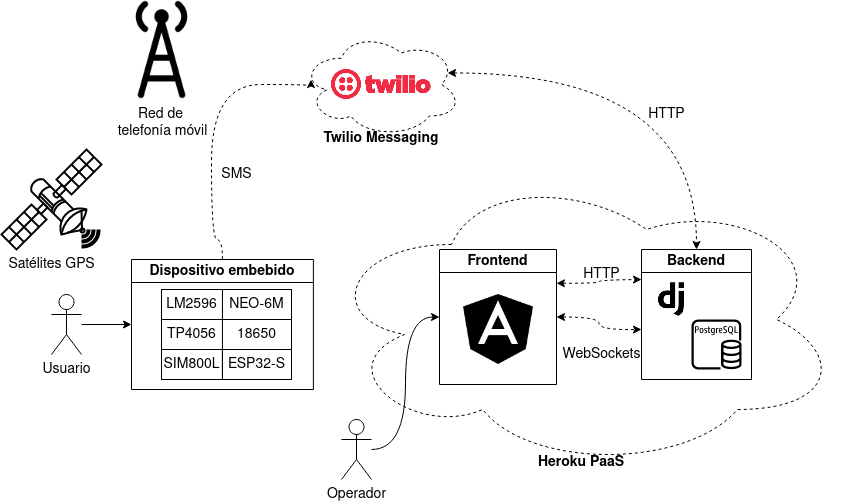
\includegraphics[width=1\textwidth]{./Figures/arquitectura.png}
	\caption{Arquitectura general del sistema}
	\label{fig:texmaker}
\end{figure}


Se pueden identificar los siguientes componentes:
\begin{itemize}
	\item En primer lugar, se observa a un usuario del dispositivo embebido, que es el componente que envía alertas mediante SMS hacia el servicio en la nube de Twilio.
	\item En segundo lugar, se encuentra el servicio de Twilio, que recepciona los mensajes recibidos y los reenvía mediante un \textit{webhook} hacia el servicio web o \textit{backend}. La comunicación entre el dispositivo embebido y Twilio fue posible ya que en este último se contrató un número teléfonico para la recepción de los SMS. 
	\item En tercer lugar, el \textit{backend}, que es el componente encargado de la recepción de alertas, procesamiento y almacenamiento de datos y comunicación con el \textit{frontend}. Fue desarrollado con el \textit{framework} Django, en Python.
	\item A continuación, se ubica el \textit{frontend}, que es la aplicación web que se encarga de toda la interacción del usuario operador con el sistema, incluyendo carga de datos y gestión de alertas. Consiste en una \textit{Single Page Application } y su desarrollo fue realizado en Angular, cuyo lenguaje es TypeScript\citep{ANGULAR:1}.
	\item Por último lugar, se encuentra un componente menor, pero no menos importante que es la base de datos encargada de almacenar toda la información del sistema, como usuarios, alertas, tipos de alertas, entre otros. El motor elegido fue PostgreSQL, descrito en el capítulo anterior.
\end{itemize}

Además, todos los \textit{endpoints} requieren de autenticación y autorización por parte del operador, a excepción de algunos que deben ser públicos para ser utilizados.
   
\section{Desarrollo de módulos de hardware}

El firmware del dispositivo embebido fue desarrollado con el \textit{Espressif IoT Development Framework}, abreviado como \textit{ESP-IDF}, el framework oficial de la placa de desarrollo elegida para el proyecto, ESP32-S\citep{ESPIDF:1}. Su lenguaje de programación es C y provee un robusto conjunto de bibliotecas para el desarrollo sobre periféricos y funcionalidades del ESP32. Adicionalmente, ESP-IDF funciona como registro de un conjunto de componentes realizados por el fabricante oficial o la comunidad para extender funcionalidades comunes de los sistemas embebidos. 

Como placa de desarrollo, el firwmare se desarrolló para una placa de desarrollo ESP32-WROOM-32s del fabricante NodeMCU, un kit de desarrollo atractivo por su bajo costo, interoperabilidad, documentación disponible y bajo consumo de energía. La ventaja de usar esta placa es que, además de contar con el framework ESP-IDF y todas las características descritas en el capítulo 2, permite que el firmware desarrollado pueda ser adaptado a placas de características similares, no quedando el firmware atado solamente a una alternativa.

Para el desarrollo, se importaron varias bibliotecas usadas para el desarrollo embebido. Entre estas, resulta importante destacar dos bibliotecas importantes:
\begin{itemize}
	\item \textit{libnmea}: Biblioteca que facilita la lectura de los datos recibidos del módulo GPS\citep{LIBNMEA:1}. Esto es posible ya que el NEO-6M utiliza un formato de mensajes estándar denominado NMEA\citep{NMEA:1}. La ventaja de usar \textit{libnmea} es que convierte los datos recibidos en estructuras de C, pudiendo acceder rápidamente a valores como la latitud, longitud, etc.
	\item \textit{iot-button}: Biblioteca que permite configuraciones complejas sobre botones o pulsadores\citep{BUTTON:1}. La ventaja de utilizar este componente es que permite rápidamente configurar funciones de \textit{callback} ante eventos como pulsaciones largas, sin requerir que se desarrolle lógica de control, así como también contempla inconvenientes como un \textit{debounce} o falsas pulsaciones al momento de accionar el botón\citep{DEBOUNCE:1}.
\end{itemize}

Estas dos bibliotecas fueron importadas al proyecto como \textit{managed components}, propios del registro de componentes externos de ESP-IDF\citep{ESPIDF:1}. En la tabla \ref{tab:bibliotecas-esp32} se encuentra detallado el uso que tuvo cada biblioteca importadas para el firmware.

\begin{table}[H]
	\centering
	\caption[Tabla de bibliotecas]{Bibliotecas más relevantes utilizadas}
	\begin{tabular}{l c}    
		\toprule
		\textbf{Bibilioteca} & \textbf{Uso} \\
		\midrule
		\makecell{\textit{iot\_button.h}} & \makecell{Implementación del botón pulsador y acciones \\ a tomar al momento de ser usado } 	\\
		\hline
		\makecell{\textit{nmea.h}}	 & \makecell{Lectura de mensajes NMEA recibidos por el módulo GPS} 	\\		
		\hline
		\makecell{\textit{string.c}}  & \makecell{Manipulación y transformación de cadenas de texto \\ al momento de leer mensajes recibidos de los módulos}  \\
		\hline	
		\makecell{\textit{ctype.c}}  & \makecell{Uso de funciones comunes de C \\ para trabajar sobre caracteres de texto }  \\
		\hline
		\makecell{\textit{uart.h}}	 & \makecell{Comunicación con los módulos GSM y GPS \\ mediante puerto serie}	\\
		\hline	
		\makecell{\textit{esp\_system.h}} &  Funciones básicas del ESP-IDF\\
		\hline
		\makecell{\textit{esp\_log.h}} &  Visualización de errores y mensajes de \textit{debug} del firmware \\
		\hline
		\makecell{\textit{esp\_pm.h} \\ \textit{esp\_sleep.h}} & Configuraciones de ahorro de energía \\
		\hline
		\makecell{\textit{adc\_oneshot.h} \\ \textit{adc/adc\_cali.h} \\ \textit{adc\_cali\_scheme.h}}  & \makecell{Conversión del módulo analógico-digital y lectura \\ de valores para calcular la carga de la batería} \\
		\hline
		\makecell{\textit{nvs.h} \\ \textit{nvs\_flash.h}} &  \makecell{Almacenamiento \textit{flash} para guardar datos  en la \\ memoria no volátil, como la última posición válida} \\
		\hline
		\makecell{\textit{freertos/FreeRTOS.h}} & Configuración del sistema operativo en tiempo real \\
		\hline
		\makecell{\textit{freertos/task.h}} & Implementación de procesos/tareas \\
		
		\bottomrule
		\hline
	\end{tabular}
	\label{tab:bibliotecas-esp32}
\end{table}

Para el desarrollo, compilación, pruebas y monitoreo, se trabajó con el entorno de desarrollo integrado Visual Studio Code, en conjunto con la extensión oficial de ESP-IDF, el cual facilita el trabajo con el kit de desarrollo y la incorporación y uso de módulos propios del ecosistema del ESP32. En la figura \ref{fig:esp32:diagrama} se pueden observar los componentes físicos del dispositivo embebido:


\begin{figure}[H]
	\centering
	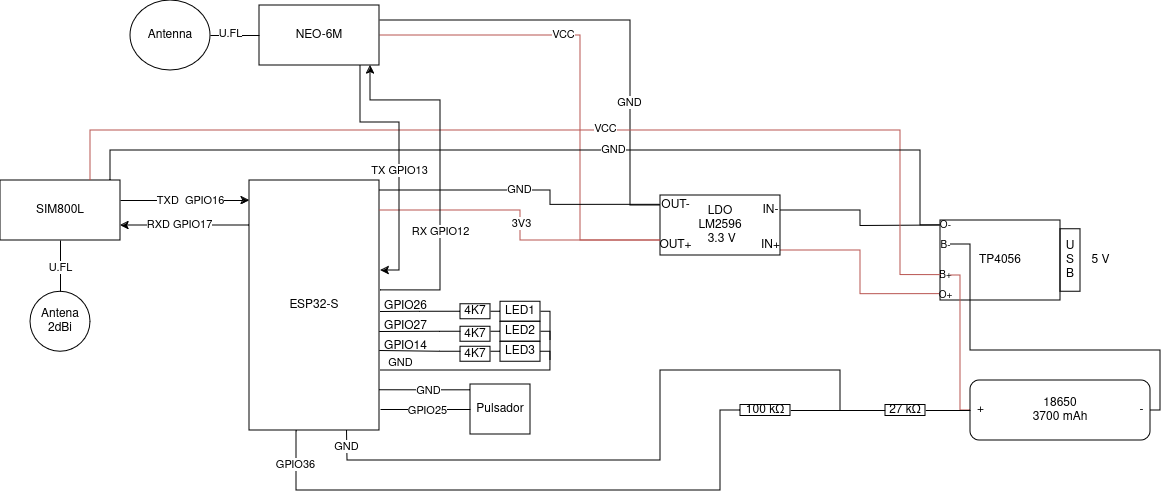
\includegraphics[width=1\textwidth]{./Figures/esp32-arquitectura.png}
	\caption{Esquema de componentes de hardware del ESP32}
	\label{fig:esp32:diagrama}
\end{figure}

Adicionalmente a los dispositivos originalmente elegidos, se incorporó un regulador de tensión LM2596 en la entrada de energía de la batería no contemplado originalmente, que permite adecuar el voltaje de entrada de 4.2 V a 3.3 V\citep{LM2596:1}, requeridos por el ESP32 y el NEO-6M. Además, se incorporó una antena activa para el módulo GPS ya con una antena pasiva la precisión de la localización obtenida era baja o tomaba más tiempo del esperado. Por otra parte, se reemplazó la antena helicoidal del módulo GSM por una con formato PCB y 3dBi de ganancia. Se muestra a continuación, en la figura \ref{fig:esp32:fisico} la implementación física del prototipo en una placa de pruebas:

\begin{figure}[H]
	\centering
	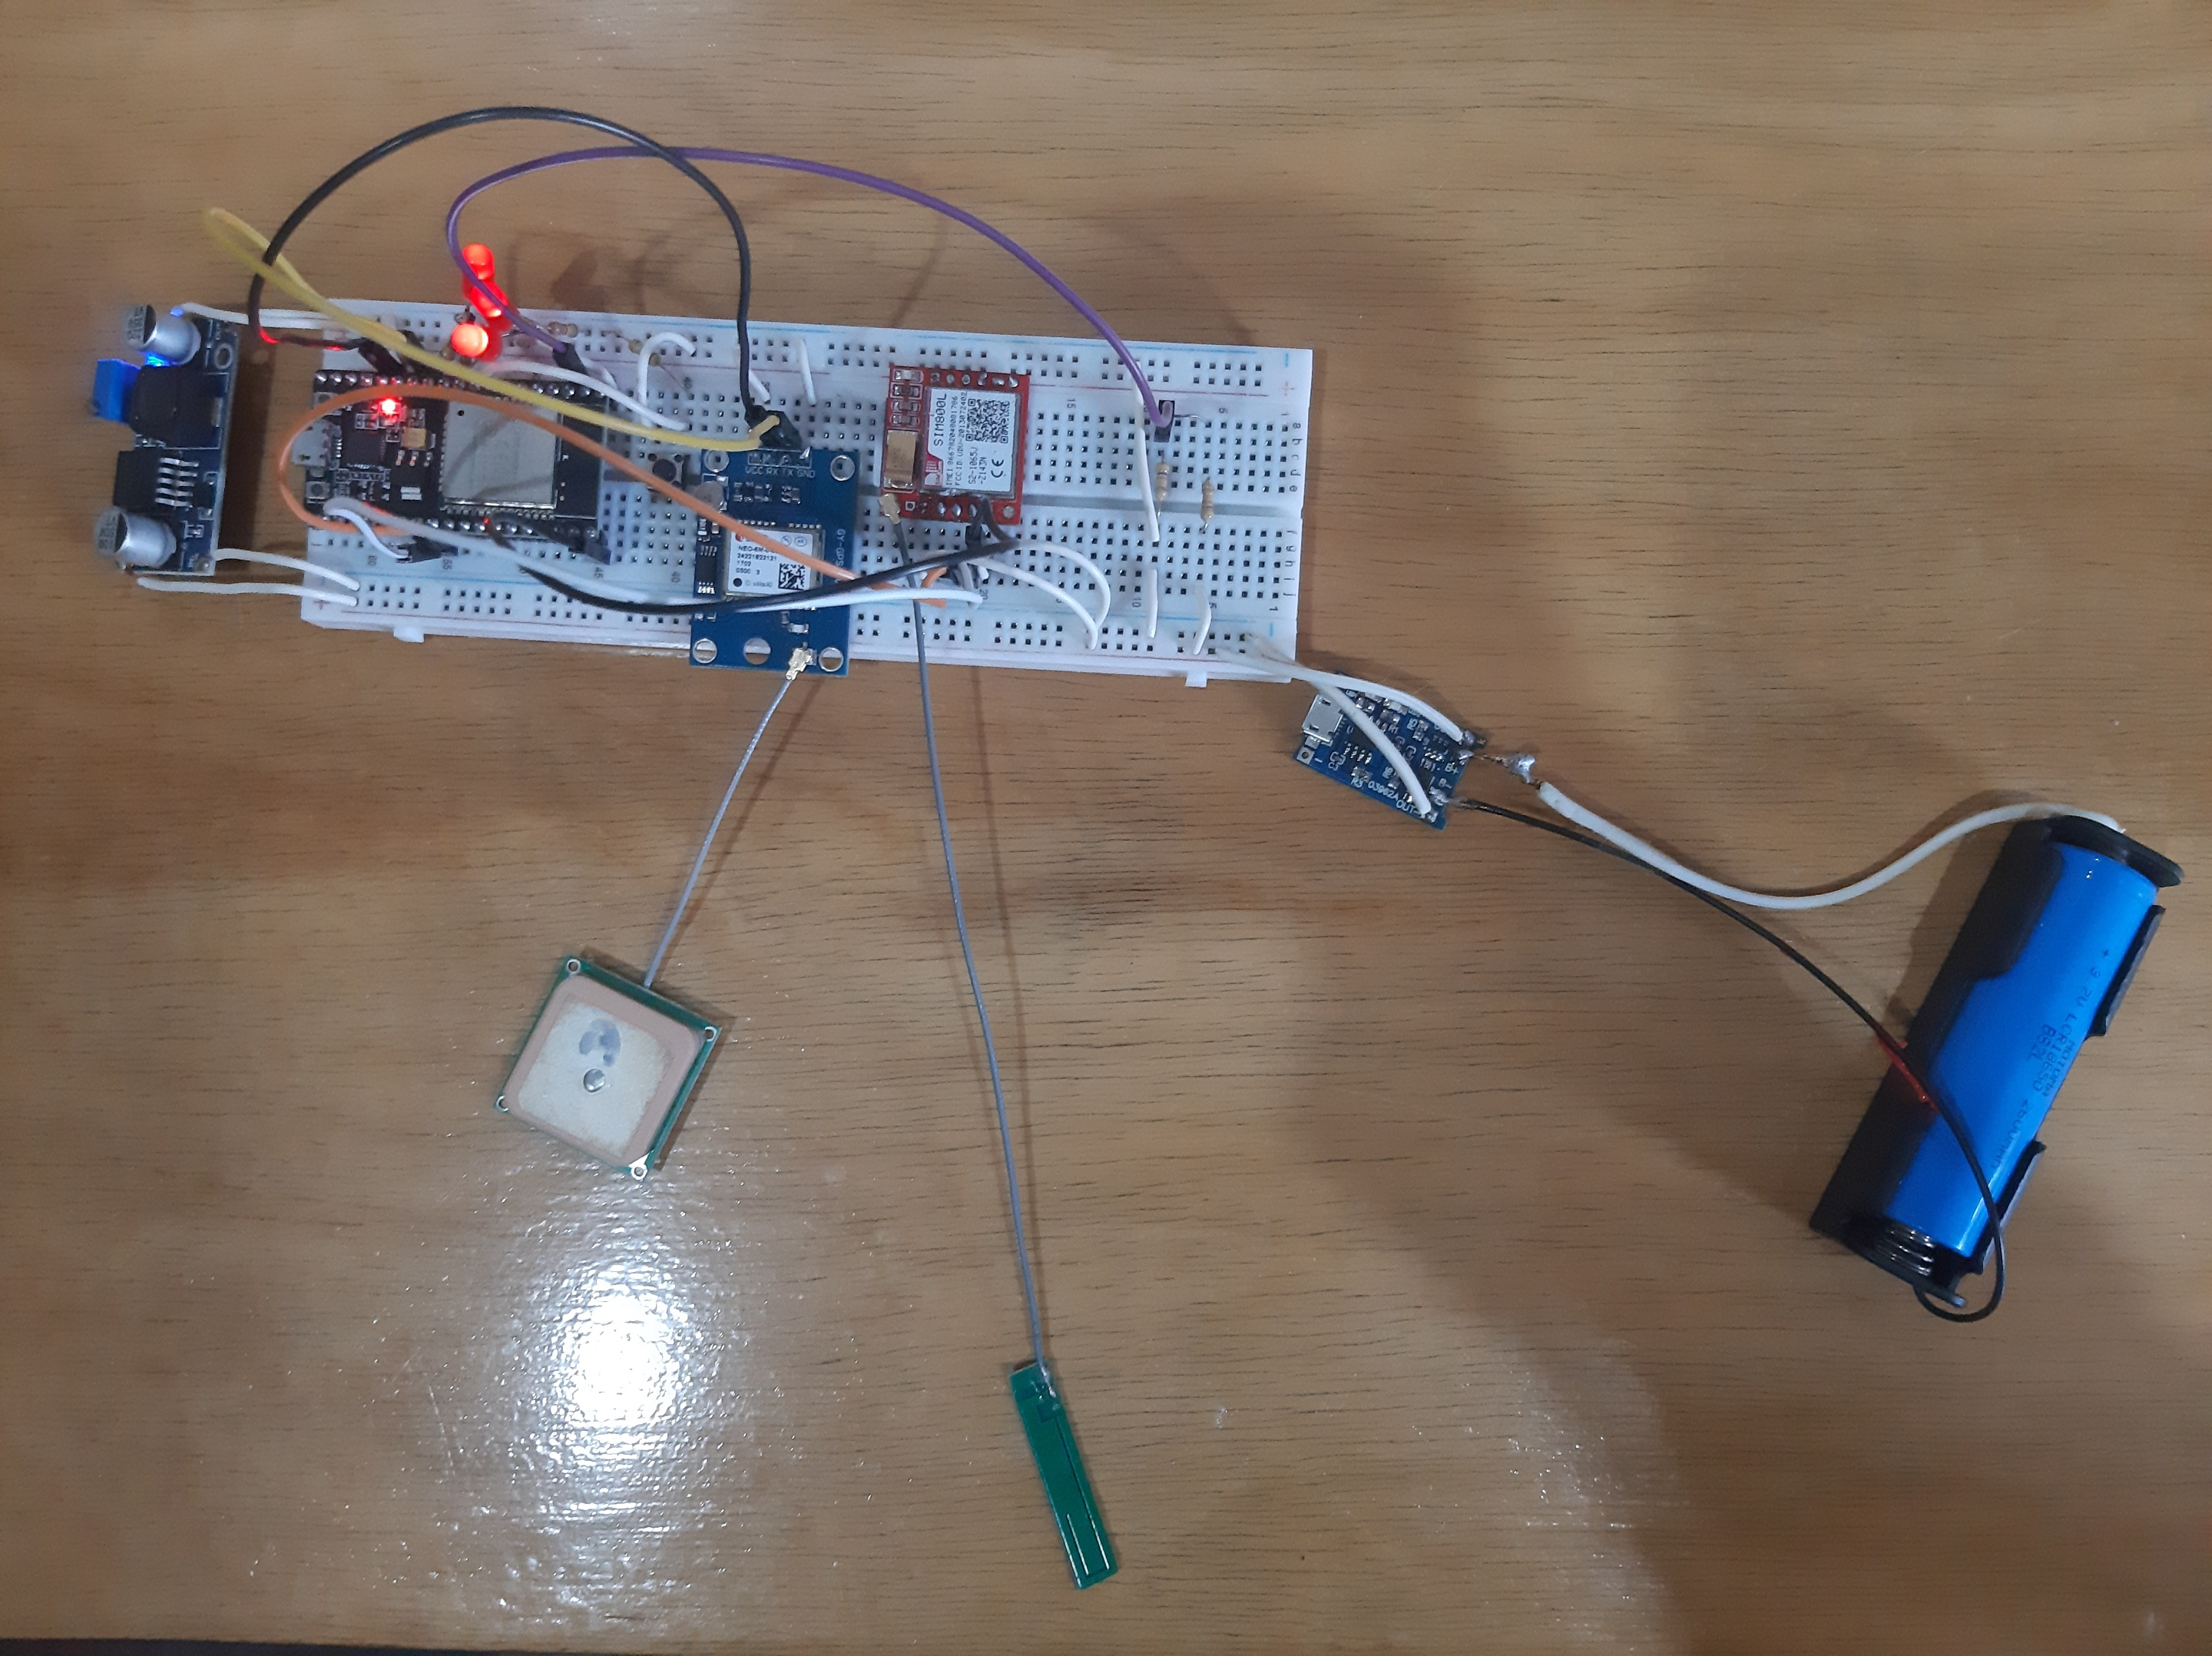
\includegraphics[width=1\textwidth]{./Figures/esp32-fisico.jpg}
	\caption{Esquema de componentes de hardware del ESP32}
	\label{fig:esp32:fisico}
\end{figure}


\subsection{Tareas del dispositivo embebido}

Para implementar las funciones del dispositivo embebido, se dividió el desarrollo del firmware en 7 bloques o funciones de código principales. Estas se pueden describir de la siguiente forma:

\begin{itemize}
	\item Inicio: consiste en la función de arranque del firmware, en donde se realizan acciones como inicialización de periféricos, revisión de errores de arranque, reducción de la velocidad de reloj del procesador al mínimo requerido, asignación inicial de variables, y por último, la configuración de las tareas que corren en bucle. Posterior al inicio, esta función finaliza su ejecución. En la figura \ref{fig:esp32:tasks1} se pueden observar todos los pasos contemplados. No es una tarea en el sentido estricto de \textit{FreeRTOS}.
	\item Manejador del módulo GSM: consiste en una función con un bucle infinito que se encarga de cada pocos segundos recibir comandos/respuestas del módulo SMS leyendo el puerto serie y tomar una acción ante cada mensaje si corresponde. En la figura \ref{fig:esp32:tasks1} se puede visualizar el bucle con las acciones que realiza. Los mensajes manejados son:
		\begin{itemize}
			\item \texttt{AT}: mensaje que representa un OK.
			\item \texttt{CMT}: mensaje que significa que se recibió un SMS; esto se utiliza para configurar el número de teléfono al cual se le deben enviar las alertas por SMS.
			\item \texttt{CMGS}: mensaje que significa se envió correctamente un SMS; se utiliza para confirmar el envío correcto de una alerta.
			\item \texttt{CSQ}: mensaje que incluye el nivel de calidad de la señal de telefonía móvil.
			\item \texttt{GSN}: mensaje que incluye el IMEI del dispositivo; se utiliza como mecanismo de seguridad ya que el SMS de configuración de teléfono debe incorporar los primeros dígitos del IMEI como validación.		
		\end{itemize}
		\item Manejador del módulo GPS: consiste en una función con un bucle que se encarga de recibir comandos/respuestas del módulo GSM leyendo el puerto serie y guardar la información recibida. Existen diferentes tipos de mensajes, pero para los fines del registro de la localización, solamente se está guardado la información del tipo de mensaje \textit{GPGGA}, que informa la posición actual y datos de los satélites\citep{NMEA:2}. En la figura \ref{fig:esp32:tasks1} se puede visualizar el bucle con las operaciones.
		\begin{figure}[H]
	\centering
	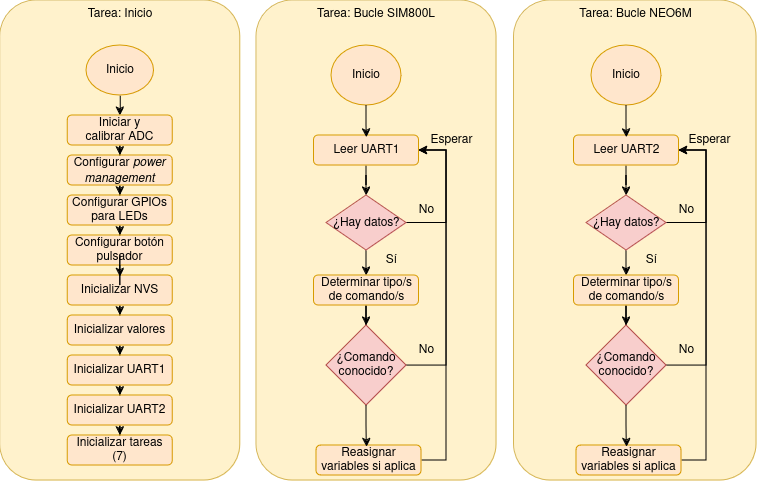
\includegraphics[width=0.95\textwidth]{./Figures/esp32-tasks1.png}
	\caption{Diagramas de flujo de tarea inicial, y bucles del módulo GSM y GPS}
	\label{fig:esp32:tasks1}
\end{figure}
		\item \textit{Setup} de energía del módulo GSM: tarea que espera por la correcta inicialización del módulo GSM y posteriormente, aplica algunas optimizaciones de energía. En la figura \ref{fig:esp32:tasks2} se listan los pasos ejecutados. Luego, la tarea termina su ejecución.
		\item \textit{Setup} de energía del módulo GPS: tarea que espera por la inicialización del módulo GPS y comunicación con al menos 5 satélites para enviarle algunos comandos de optimización. Luego de esto, la tarea finaliza. En la figura \ref{fig:esp32:tasks2} se pueden visualizar el flujo de esta.
		\begin{figure}[H]
	\centering
	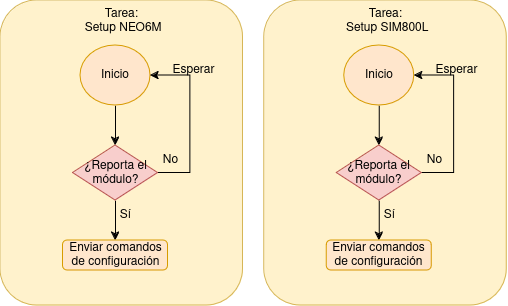
\includegraphics[width=0.75\textwidth]{./Figures/esp32-tasks2.png}
	\caption{Diagramas de flujo de las tareas de \textit{setup} de energía}
	\label{fig:esp32:tasks2}
\end{figure}

		\item Control de estado de GPS, GSM y batería: esta tarea tiene como objetivo, cada 30 segundos, leer el estado de las variables de calidad de la señal GSM, cantidad de satélites conectados y nivel de batería, y parpadear 3 luces dependiendo del estado de estas variables. En el desarrollo, se repartió en tres funciones pequeñas, pero a fines explicativos se presenta como una única tarea. En la figura \ref{fig:esp32:tasks3} se puede observar el flujo de ejecución de la tarea.
		\item Almacenamiento períodico de datos: cada 1 minuto esta tarea se encarga de leer las variables de latitud, longitud, IMEI y número de teléfono asignado y almacenarlas en el almacenamiento no volátil. en el caso de que los valores fueran válidos. En la figura \ref{fig:esp32:tasks3} se puede observar el bucle ejecutado por la tarea.
		\item Control períodico del módulo GSM: esta tarea se encarga de solicitarle información al módulo GSM información sobre el estado de la red cada 1 minuto. Esto es debido a que el módulo GSM no reporta automáticamente su estado, a diferencia del módulo GPS que si lo hace.  En la figura \ref{fig:esp32:tasks3} se puede apreciar el control que realiza la función.
		
	\begin{figure}[H]
		\centering
		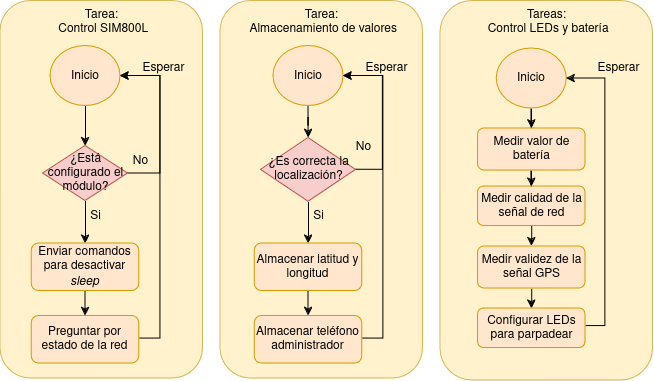
\includegraphics[width=0.9\textwidth]{./Figures/esp32-tasks3.png}
		\caption{Diagramas de flujo de las tareas de control y almacenamiento}
		\label{fig:esp32:tasks3}
	\end{figure}

\end{itemize}

Por último, se puede considerar una última función más dentro del firmware que es el interruptor ante la pulsación del botón activador. En caso que se supere un umbral de 3 segundos del pulsador presionado, se activará \textit{callback} definido para ese evento. Este evento se encarga de levantar los valores actuales de la última localización válida almacenada, determinar cual es el número de teléfono al cual se debe enviar el mensaje de alerta y enviar los comandos hacia el módulo GSM para enviar el SMS. 

En la figura \ref{esp32:callback-codigo} se muestra un diagrama de flujo resumido de la operatoria de la interrupción. Para la asociación del \textit{callback} con el evento, se puede ver el código definido en la función inicial del firmware en la figura \ref{fig:esp32:callback-codigo}, donde \texttt{sos\_button\_long\_press\_cb} es una función definida y \texttt{cfg} es la definición del evento.

\begin{lstlisting}[label=esp32:callback-codigo,caption=Definición del evento y asociación del \textit{callback}]  % Start your code-block
// SOS button configure
button_config_t gpio_btn_cfg = {
    .type = BUTTON_TYPE_GPIO,
    .long_press_time = SOS_BUTTON_LONG_PRESS_TIME_MS,
    .gpio_button_config = {
        .gpio_num = SOS_BUTTON,
        .active_level = 1,
        .enable_power_save = true},
};

button_handle_t gpio_btn = iot_button_create(&gpio_btn_cfg);
if (NULL == gpio_btn)
{
    ESP_LOGE(TAG, "Button create failed");
}

button_event_config_t cfg = {
    .event = BUTTON_LONG_PRESS_START,
    .event_data.long_press.press_time = SOS_BUTTON_LONG_PRESS_TIME_MS,
};

ESP_ERROR_CHECK(iot_button_register_event_cb(gpio_btn, cfg, sos_button_long_press_cb, NULL));

\end{lstlisting}

\begin{figure}[H]
	\centering
	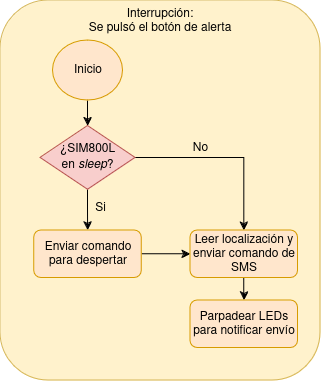
\includegraphics[width=0.5\textwidth]{./Figures/esp32-callback.png}
	\caption{Diagrama de flujo del \textit{callback} por pulsación}
	\label{fig:esp32:callback-codigo}
\end{figure}


\subsection{Optimizaciones de energía aplicadas}

Se aplicaron diferentes técnicas de optimización sobre el ESP32-S y los módulos GSM y GPS con el objetivo de optimizar y disminuir el consumo de energía:
\begin{itemize}
	\item Se configuró \textit{FreeRTOS} para solamente utilizar un núcleo del ESP32-S.
	\item Se limitó la frecuencia del procesador para solamente utilizar como máximo 80 MHz.
	\item Se desactivaron todos los periféricos no usados, como WiFi, Bluetooth, etc.
	\item Se configuró el \textit{Dynamic frequency scaling} o DFS del ESP32, que permitiría que se reduzca la velocidad del reloj del procesador\citep{ESP32:2}.
	\item Se configuró el modo \textit{sleep} del módulo SIM800L, desactivandolo solo cuando se le debe enviar comandos.
	\item Se desactivó el LED de notificación de calidad de señal del módulo SIM800L, ya que la comprobación se realiza de forma programática.
	\item Se redujo la frecuencia de actualización de mensajes del módulo NEO-6M hacia el ESP32.
	\item Se aplicó sobre NEO-6M una configuración de energía denominada \textit{Power Save Mode} para reducir la frecuencia de actualización hacia los satélites GPS\citep{NEO6M:2}.
	\item Se configuró el modo \textit{sleep} del módulo SIM800L, desactivandolo solamente cada ciertos intervalos de tiempo.
	\item Se utilizaron tiempos muertos de espera o \textit{standy} del orden de varios segundos en el ESP32-S, resultando en que gran parte del tiempo, la placa se encuentre en espera.
	\item Se redujo el consumo de energía de los 3 LEDs indicadores de GSM, GPS y batería mediante la incorporación de resistencias, requiriendo aproximadamente 1 mA para todos los LEDs.
\end{itemize}

Además, se intentó aplicar un manejo tanto manual como automático (configurable mediante el uso de DFS) del modo \textit{light sleep} pero se encontró que, después de varios intentos y pruebas, el consumo de energía no disminuyó. Se interpretó, en base a las pruebas durante el desarrollo, que es debido a características de fabricación del modelo ESP32-WROOM-32s de NodeMCU. Se midió un consumo en \textit{idle} de aproximadamente 15 mA, aunque esté en \textit{deep sleep} o \textit{light sleep}.

\section{Desarrollo de módulo de backend}

El \textit{backend} fue desarrollado con el framework Django y Python. Para todas las funcionalidades, se estructuró el proyecto siguiendo los lineamientos de Django, que consiste en principalmente dividir la aplicación en módulos web por temática o características. Para el caso de esta aplicación, se identificaron dos módulos:
\begin{itemize}
	\item \textit{Users}: para englobar toda la funcionalidad referida a usuarios.
	\item \textit{Alerts}: para englobar toda la funcionalidad referida a beneficiarios y alertas.
\end{itemize}

Esto no significa que no puedan o no deban referenciarse los módulos entre sí, sino que es una forma lógica de estructurar la información perteneciente a la misma lógica de negocio. En la figura \ref{backend:folder1} y \ref{backend:folder2} se pueden visualizar las carpetas de cada módulo con sus respectivos componentes.

\begin{figure}[H]
\centering
\begin{minipage}{.5\textwidth}
  \centering
  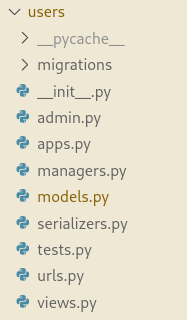
\includegraphics[width=.4\linewidth]{./Figures/backend-folder1.png}
  \captionof{figure}{Estructura de archivos de módulo de \textit{Users}}
  \label{backend:folder1}
\end{minipage}%
\begin{minipage}{.5\textwidth}
  \centering
  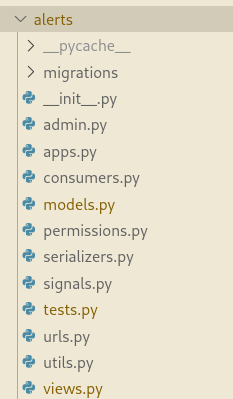
\includegraphics[width=.4\linewidth]{./Figures/backend-folder2.png}
  \captionof{figure}{Estructura de archivos de módulo de \textit{Alerts}}
  \label{backend:folder2}
\end{minipage}
\end{figure}

Para la implementación, se incorporaron varias bibliotecas externas, cuyo aporte se muestra en la tabla \ref{backend:libraries}:

\begin{table}[H]
	\centering
	\caption[Tabla de bibliotecas]{Bibliotecas externas más relevantes}
	\begin{tabular}{l c}    
		\toprule
		\textbf{Bibilioteca} & \textbf{Uso} \\
		\midrule
		\makecell{\textit{djangorestframework}}	 & \makecell{Biblioteca de Django para \\ el desarrollo de APIs REST} 	\\		
		\hline
		\makecell{\textit{psycopg}}  & \makecell{Biblioteca para conexión a PostgreSQL\citep{DJANGO:4}}  \\
		\hline	
		\makecell{\textit{django-twilio}}  & \makecell{Biblioteca oficial de Twilio\citep{DJANGO:3} \\ para comunicación con \textit{Twilio Messaging Services} }  \\
		\hline
		\makecell{\textit{channels}}	 & \makecell{Biblioteca para la implementación \\ de WebSockets en Django\citep{DJANGO:5}}	\\
		\hline	
		\makecell{\textit{djangorestframework-simplejwt}} &  \makecell{Biblioteca para el \textit{middleware}  \\ de autenticación mediante tokens JWT} \\
		\hline
		\makecell{\textit{drf\_yasg}} &  \makecell{Biblioteca para generar \\ documentación de API en Swagger} \\
		\hline
		\makecell{\textit{uvicorn}} & Servidor web ASGI para Python\citep{DJANGO:7} \\
		\hline
		\makecell{\textit{django-cors-headers}}  & \makecell{\textit{Middleware} para incorpora  \\ encabezados en las peticiones de la API} \\
		\hline
		\makecell{\textit{dj-database-url}} &  \makecell{Biblioteca para conectarse \\ a base de datos PostgreSQL de Heroku} \\
		\hline
		\makecell{\textit{django-channels-jwt}} & \textit{Middleware} para autenticación de WebSockets \\
		\bottomrule
		\hline
	\end{tabular}
	\label{backend:libraries}
\end{table}


En la figura \ref{backend:modulos} se presenta en forma de diagrama de bloques los principales componentes de la API:

\begin{figure}[H]
	\centering
	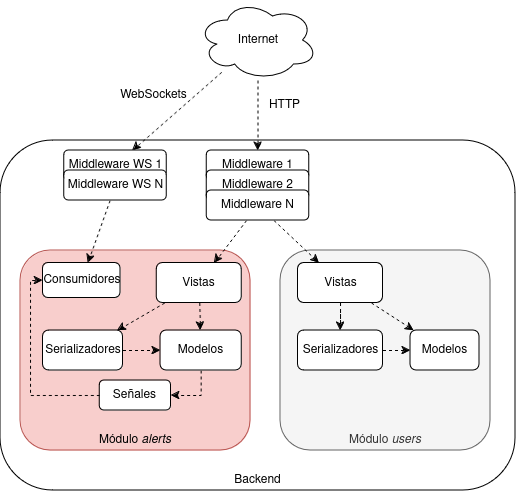
\includegraphics[width=0.9\textwidth]{./Figures/backend-componentes.png}
	\caption{Diagrama en bloques del \textit{backend}}
	\label{backend:modulos}
\end{figure}

Se describen a continuación los componentes de mayor relevancia de los módulos:

\begin{itemize}
	\item Modelos: clases que representan los modelos de datos, como pueden ser las entidades de una alerta y un beneficiario.
	\item Serializadores: clases que agrupan la lectura, escritura, validación y salida de modelos de datos. Los serializadores permiten encapsular lógica de validación para diferentes operaciones o adaptar la representación de los datos según la necesidad\citep{DJANGO:8}. En la figura \ref{backend:serializer1} se muestra el serializador de la entidad \textit{Beneficiary} junto con validaciones y acciones que deben realizarse durante la creación y actualización, así como también definir restricciones al momento de realizar la carga de datos.
	\begin{figure}[H]
	\centering
	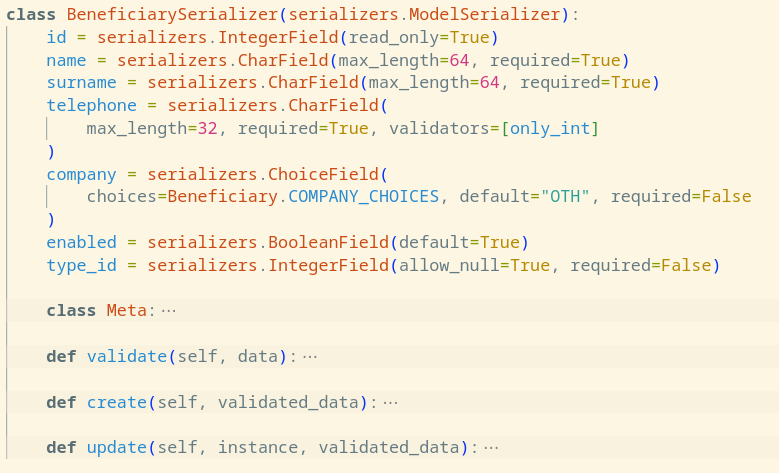
\includegraphics[width=0.75\textwidth]{./Figures/backend-serializer1.png}
	\caption{Serializador de la entidad \textit{Beneficiary}}
	\label{backend:serializer1}
    \end{figure}
	\item Vistas: clases que engloban peticiones HTTP sobre entidades o clases para atender un único tipo de petición, dependiendo del requerimiento\citep{DJANGO:9}. En la figura \ref{backend:view1} se puede apreciar la definición del \textit{ViewSet} de la clase \textit{Beneficiary}, pudiendo observarse que se asignaron de forma declarativa los permisos requeridos para realizar las peticiones, y los filtros habilitados, sin requerir código adicional.
		\begin{figure}[H]
	\centering
	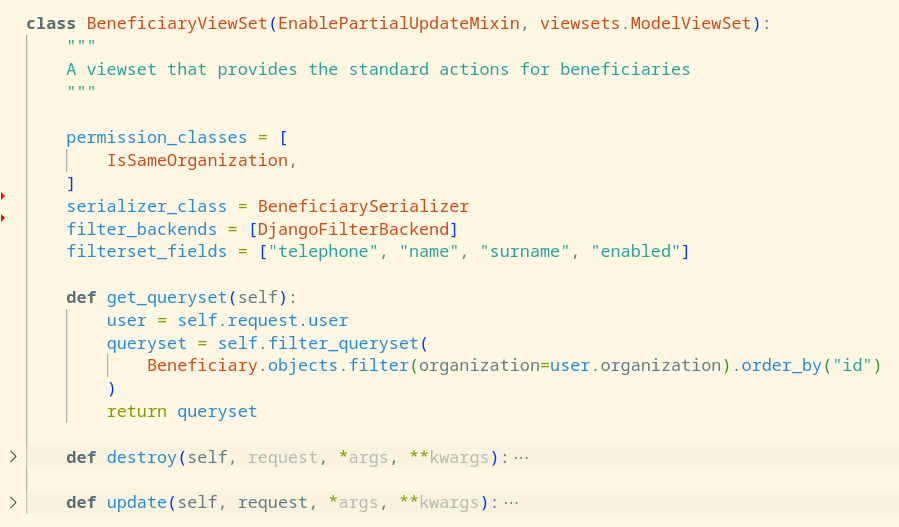
\includegraphics[width=0.75\textwidth]{./Figures/backend-view1.png}
	\caption{Serializador de la entidad \textit{Beneficiary}}
	\label{backend:view1}
    \end{figure}
    \item Consumidores: representa un servicio de WebSockets que permite obtener una alerta entrante en tiempo real.
    \item \textit{Middlewares}: clases que permiten interceptar peticiones hacia la API\citep{DJANGO:10} y realizar comprobaciones como ver el rol del usuario, o que este tenga la correcta autorización en las peticiones. No se desarrolló ningún \textit{middleware} sino que se utilizaron bibliotecas externas ya provistas.
    \item Señales: hace referencia a una notificación que se genera dentro de la aplicación ante un evento\citep{DJANGO:11}. En el marco de esta aplicación, cuando se almacena una nueva alerta, se genera una señal que notifica en tiempo real mediante \textit{WebSockets} el dato creado.
\end{itemize}

Respecto a las características, se diseñó el \textit{backend} con la idea de un producto \textit{multitenant}, es decir que permita que a futuro existan diferentes organizaciones cliente dentro de este\citep{DJANGO:12}. Debido a esta característica, todos los datos están contenidos dentro de una misma organización, compartida por los usuarios, beneficiarios, entre otros datos cargados. En la figura \ref{backend:modelo} se puede visualizar el modelo de datos relacional con las entidades diseñadas.

\begin{figure}[H]
	\centering
	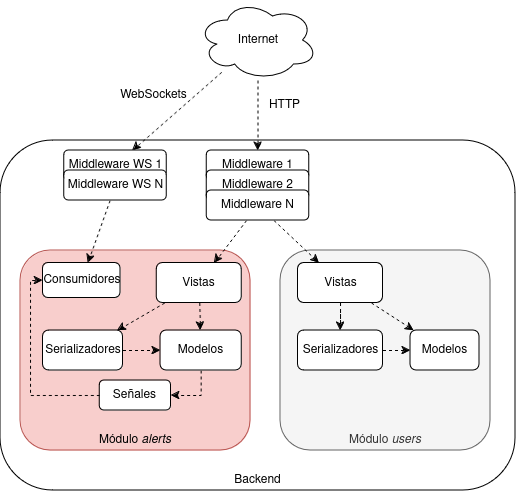
\includegraphics[width=0.75\textwidth]{./Figures/backend-modelos.png}
	\caption{Modelo de datos}
	\label{backend:modelo}
\end{figure}


De todas maneras, para esta versión inicial, solo se contempla un usuario por organización en el \textit{frontend}, aunque a futuro el diseño y la lógica de negocio en la API se encuentra desarrollada para contemplar una organización con un usuario raíz o padre y un conjunto de usuarios operadores, de menor privilegio.

\subsection{Servicios desarrollados}

A continuación, se muestran en la tabla \ref{tab:endpoints} los servicios implementados:

\begin{table}[H]
	\centering
	\caption[\textit{Servicios}]{\textit{Endpoints} implementados}
	\begin{tabular}{l c c}    
		\toprule
		\textbf{\textit{Endpoint}} 	 & \textbf{Descripción} \\
		\midrule
		GET /alert-types/ & Obtener tipos de alerta  \\		
		POST /alert-types/& Crear un tipo de alerta		\\		
		GET /alert-types/{id}/ & Obtener un tipo de alerta \\
		PUT /alert-types/{id}/ & Editar un tipo de alerta		\\
		DELETE /alert-types/{id}/ & Eliminar un tipo de alerta  \\
		\hline
		GET /alerts/ & Obtener alertas  \\		
		GET /alerts-summary/ & Obtener alertas de las últimas 24 horas \\		
		GET /alerts/{id}/ & Obtener una alerta \\
		PUT /alerts/{id}/ & Editar una alerta		\\
		PATCH /alerts/{id}/ & Editar parcialmente una alerta   \\
		\hline
		GET /beneficiaries/ & Obtener beneficiarios  \\			
		GET /beneficiaries/{id}/ & Obtener un beneficiario \\
		PUT /beneficiaries/{id}/ & Editar un beneficiario		\\
		PATCH /beneficiaries/{id}/ & Editar parcialmente un beneficiario   \\
		DELETE /beneficiaries/{id}/ & Desactivar un beneficiario \\
		\hline
		GET /beneficiary-types/ & Obtener tipos de beneficiarios  \\			
		GET /beneficiary-types/{id}/ & Obtener un tipo de beneficiario \\
		PUT /beneficiary-types/{id}/ & Editar un tipo de beneficiario		\\
		DELETE /beneficiary-types/{id}/ & Desactivar un beneficiario \\
		\hline
		POST /users/admin/ & \makecell{Crear un usuario administrador \\ con una organización}  \\			
		GET /user-details/ & Obtener datos del usuario \\
		PATCH /user/{id}/ & Editar parcialmente un usuario \\
		\hline
		POST /login/ & Realizar login programático \\	
		GET /ws-auth/ & \makecell{Obtener token efímero para \\ conexión a WebSockets} \\
		POST /twilio-webhook/ & \makecell{Webhook para generar una \\ alerta desde Twilio} \\	
		WS /ws/alerts/organization-{id}/ & Conectarse a canal de WebSockets	\\
		\bottomrule
		\hline
	\end{tabular}
	\label{tab:endpoints}
\end{table}

Todos estos servicios fueron documentados mediante Swagger, una herramienta para documentación de APIs\citep{DJANGO:6}. Todas las vistas, a excepción del registro de un nuevo usuario administrador, requieren de autenticación mediante un token JWT. Esto es autogestionado mediante la incorporación de un \textit{middleware} de Django, sin requerir código adicional más allá de declarar en la configuración de Django de la aplicación, que \textit{middlewares} utilizar para la autenticación, como se observa en la figura \ref{backend:settings1}:

\begin{figure}[H]
	\centering
	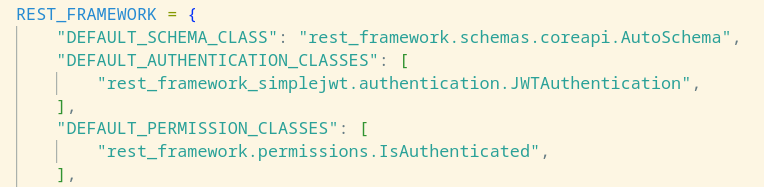
\includegraphics[width=0.5\textwidth]{./Figures/backend-settings1.png}
	\caption{Configuración de \textit{middlewares} para la autenticación de la API}
	\label{backend:settings1}
\end{figure}



\section{Desarrollo de módulo de frontend}

\section{Integración}

Resulta importante destacar que toda la interacción entre el \textit{backend} y \textit{frontend} es realizada mediante \textit{endpoints} HTTP y \textit{WebSockets} para comunicación en tiempo real, utilizando TLS/SSL para securizar las conexiones. 

Por el lado del despliegue, los componentes web se desplegaron en la nube de Heroku mediante el uso de \textit{dynos} básicos, que son contenedores de aplicaciones web\citep{HEROKU:1}, y para la base de datos, se utilizó un \textit{addon} de PostgreSQL, que consiste en un complemento que permite incorporar una base de datos como SaaS u otros componentes requeridos por los sistemas, como pueden ser bases de datos en memoria o brókers\citep{HEROKU:2}.


	% Chapter Template

\chapter{Ensayos y resultados} % Main chapter title



\label{Chapter4} % Change X to a consecutive number; for referencing this chapter elsewhere, use \ref{ChapterX}

En este capítulo se presentan y describen los ensayos llevados a cabo y las técnicas implementadas para verificar la funcionalidad de cada componente desarrollado y del sistema en su totalidad. Además, se muestran y analizan los resultados obtenidos en cada prueba.

%----------------------------------------------------------------------------------------
%	SECTION 1
%----------------------------------------------------------------------------------------

\section{Banco de pruebas}

El banco de pruebas que se utilizó para este trabajo, estuvo conformado por los elementos descritos en la tabla \ref{tab:banco-pruebas}:

\begin{table}[H]
	\centering
	\caption[\textit{Banco de pruebas}]{Elementos del banco de pruebas}
	\begin{tabular}{l c c}    
		\toprule
		\textbf{Elemento} 	 & \textbf{Aplicación} \\
		\midrule
		Computadora local & Despliegue local de \textit{frontend} y \textit{backend}  \\		
		Prototipo de hardware & Botón antipánico \\		
		Chip GSM & \makecell{Número de teléfono para el envío de  SMS en el \\ hardware} \\
		Postman & Herramienta para pruebas manuales del \textit{backend}\\
		Número de Twilio & \makecell{Número de teléfono virtual para la recepción de SMS}  \\
		Multímetro & Herramienta para medir consumo energético  \\
		CP2102 & Conversor de puerto serie a USB para \textit{debugging}\citep{CP2102:1}\\	
		\bottomrule
		\hline
	\end{tabular}
	\label{tab:banco-pruebas}
\end{table}

En relación a las pruebas a realizar para verificar el cumplimiento de los componentes desarrollados, se determinaron las siguientes:

\begin{itemize}
\item Dispositivo embebido:
	\begin{itemize}
	\item Prueba de almacenamiento de las latitud, longitud, IMEI, teléfono almacenado.
	\item Prueba de SMS de configuración de teléfono.
	\item Medición de consumo energético de módulos de hardware.
	\item Prueba de medición de carga de batería.
	\item Prueba de pulsación de botón de alerta y envío de SMS con datos de localización.
	\end{itemize}
\item \textit{Backend}:
	\begin{itemize}
	\item Prueba de creación de usuario administrador y su organización.
	\item Prueba de obtención/creación/modificación/desactivación de beneficiarios.
	\item Prueba de obtención/creación/modificación/desactivación de tipos de beneficiarios.
	\item Prueba de obtención/creación/modificación/desactivación de tipos de alertas.
	\item Prueba de obtención/actualización de alertas.
	\item Prueba de conexión a canal de \textit{WebSockets}.
	\item Prueba de recepción de alerta mediante \textit{webhook}.
	\item Prueba de bloqueo de nueva alerta para un número de teléfono no habilitado.
	\end{itemize}
\item \textit{Frontend}:
	\begin{itemize}
	\item Prueba de registro.
	\item Prueba de login.
	\item Prueba de visualización de últimas alertas recibidas.
	\item Prueba de atención de nuevas alertas.
	\item Prueba de recepción de nuevas alertas en tiempo real.
	\item Prueba de visualización/modificación/creación/eliminación de beneficiarios, tipos de beneficiarios y tipos de alerta.
	\item Prueba de visualización y exportación de alertas.
	\end{itemize}

\end{itemize}


\section{Metodología empleada}

Para poder ver los mensajes informativos del firmware, al momento de hacer pruebas, se conectó la salida del puerto UART0 del ESP32 como se observa en la figura \ref{fig:cp2102}, usado para mensajes de \textit{debug} por parte del ESP32\citep{UART:1}, al dispositivo CP2102 que permite enviar los mensajes al puerto USB de la computadora. En la figura \ref{fig:esp32:debug} se observan mensajes enviados por puerto serie. Esto es porque en las pruebas integrales, no se utilizó la alimentación por USB del ESP32, sino que se utilizó la batería, perdiendo la posibilidad de ver directamente la salida del ESP32.

\begin{figure}[H]
\centering
\begin{minipage}{.5\textwidth}
  \centering
  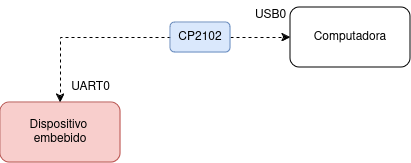
\includegraphics[width=0.9\linewidth]{./Figures/cp2102.png}
  \captionof{figure}{Esquema de conexión del CP2102}
  \label{fig:cp2102}
\end{minipage}%
\begin{minipage}{.5\textwidth}
  \centering
  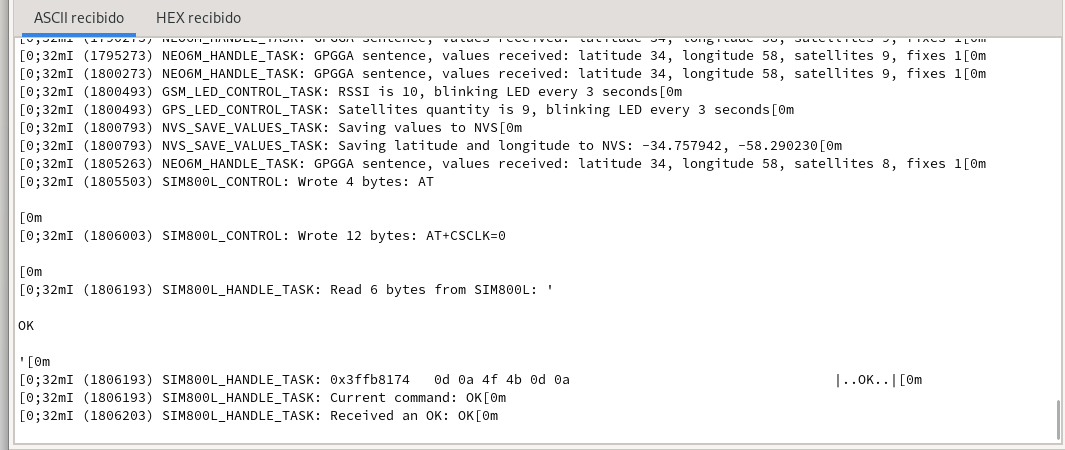
\includegraphics[width=0.9\linewidth]{./Figures/moserial-debug.png}
  \captionof{figure}{Salida del ESP32 vista en Moserial}
  \label{fig:esp32:debug}
\end{minipage}
\end{figure}

Para medir el consumo energético, se configuró el multímetro con la disposición observada en la figura \ref{fig:pruebas:multimetro}, es decir, en serie con los módulos de hardware:

\begin{figure}[H]
	\centering
	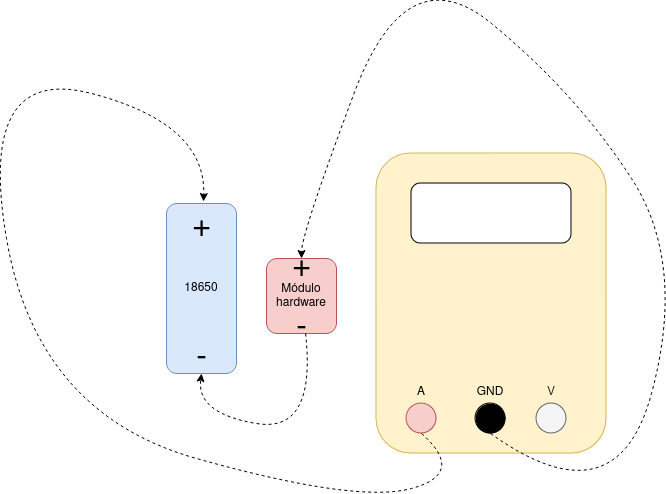
\includegraphics[width=1\textwidth]{./Figures/multimetro.png}
	\caption{Esquema de conexión del multímetro}
	\label{fig:pruebas:multimetro}
\end{figure}

Además, se contrastó en las mediciones el consumo informado por el \textit{datasheet} del fabricante de cada módulo, para determinar si efectivamente las mediciones fueron correctas. Se concluyó de que la calidad de las mediciones eran aceptables, aunque lo ideal hubiese sido contar con un osciloscopio. Por otra parte, las pruebas de consumo energético se realizaron primero de forma aislada con cada componente, y luego se midió el consumo total del dispositivo embebido. 

Es importante destacar la necesidad de haber contado con la aplicación desplegada en un entorno \textit{cloud} para las pruebas, ya que la integración con Twilio no fue posible con el despliegue local. La base de datos local se configuró utilizando una imagen Docker con PostgreSQL\citep{DOCKER:2}.

Para verificar el funcionamiento del sistema web, se implementó una cantidad de pruebas unitarias en el \textit{backend}, con la biblioteca \textit{APITestCase}, provista por el framework Django para el desarrollo de pruebas unitarias\citep{DJANGO:13}. Estas pruebas permitieron validar que la API funcionase correctamente para las operaciones básicas.

Por otra parte, se realizaron algunas pruebas de forma manual mediante el uso de Postman, herramienta para desarrollo y testing de APIs para algunos casos particulares, como:
\begin{itemize}
	\item Establecimiento de conexión mediante \textit{WebSockets}.
	\item Verificación de recepción de nuevas alertas en tiempo real mediante el canal de \textit{WebSockets}.
\end{itemize}

Para verificar el funcionamiento correcto del \textit{frontend}, se realizaron pruebas conectadas con el \textit{backend}.

\section{Pruebas de módulos de hardware}

En la figura \ref{fig:esp32:fisico} se puede visualizar la disposición física del dispositivo embebido:
\begin{figure}[H]
	\centering
	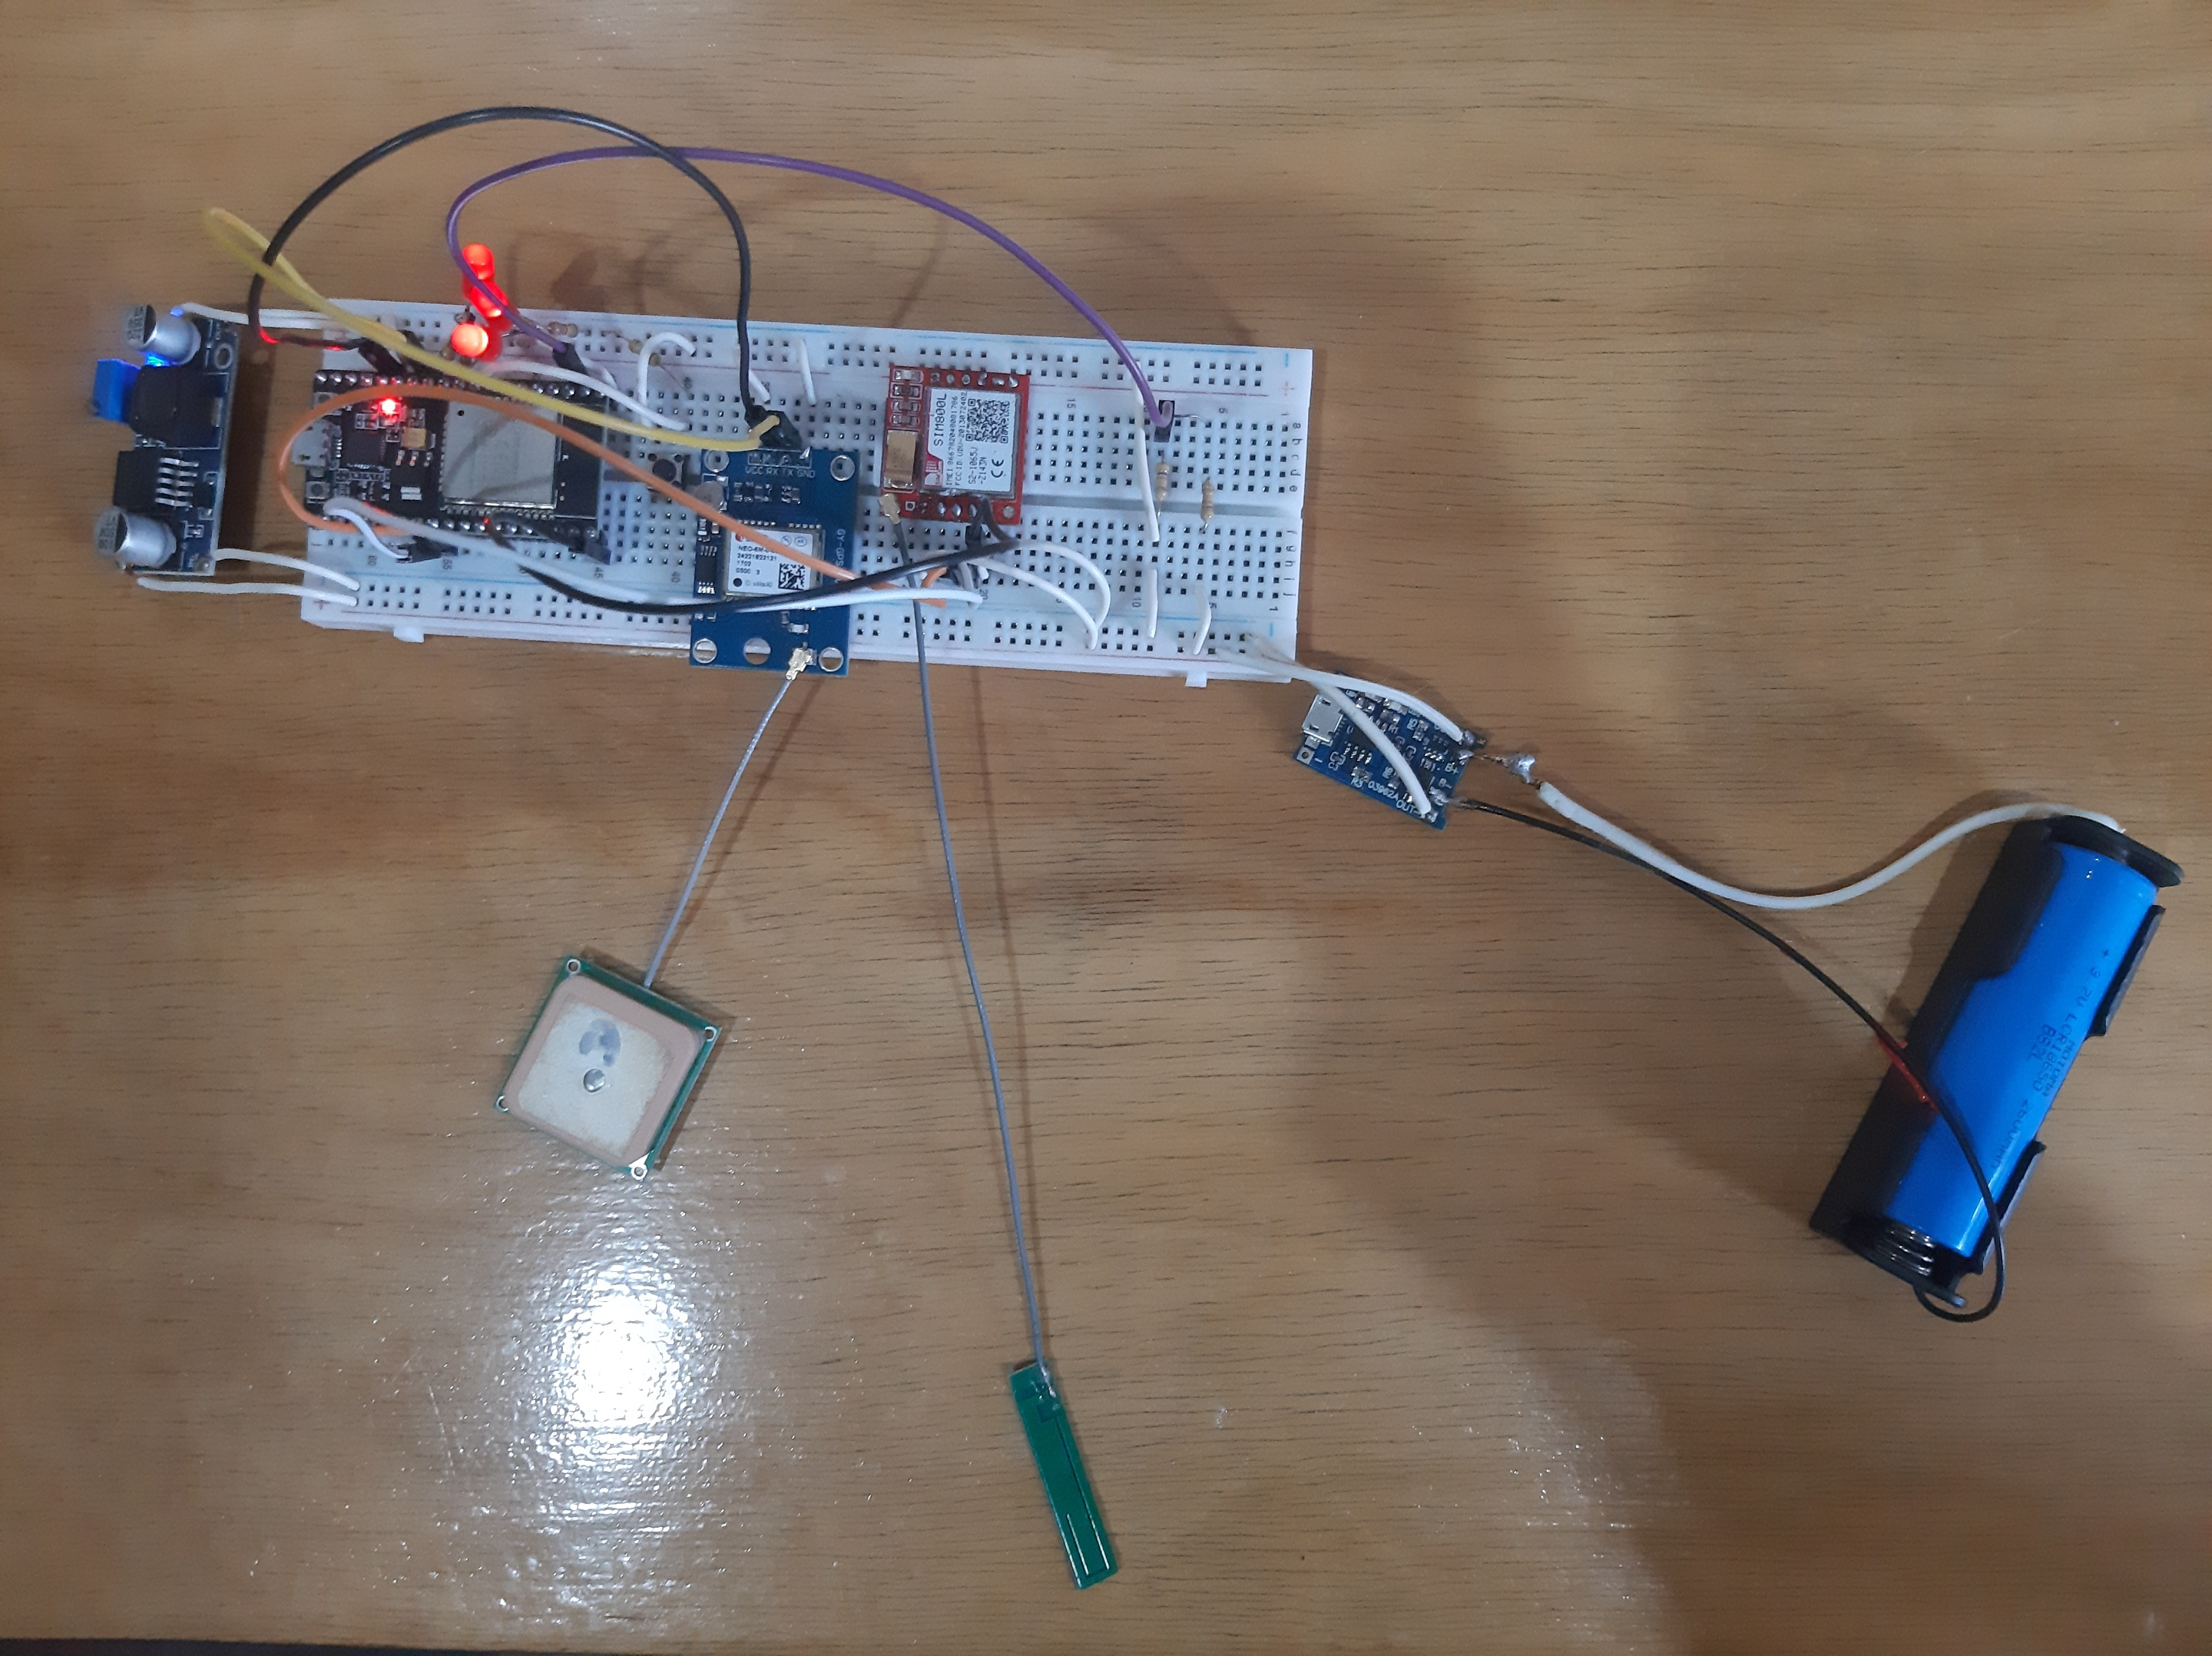
\includegraphics[width=1\textwidth]{./Figures/esp32-fisico.jpg}
	\caption{Esquema de componentes de hardware del ESP32}
	\label{fig:esp32:fisico}
\end{figure}

Respecto al almacenamiento de variables, la figura \ref{fig:esp32:nvs} muestra la lectura de variables almacenadas:

\begin{figure}[H]
	\centering
	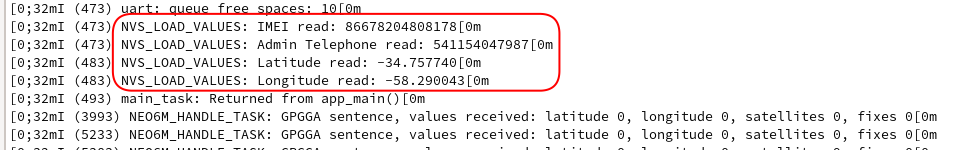
\includegraphics[width=1\textwidth]{./Figures/esp32-nvs.png}
	\caption{Lectura de variables almacenadas en el almacenamiento no volátil}
	\label{fig:esp32:nvs}
\end{figure}

De todas maneras, se encontraron inconvenientes esporádicos con las variables de latitud y longitud almacenadas, ya que cada ciertos reinicios o reinstalación del firmware, las variables en el almacenamiento no volátil se reinicializaban.

Posteriormente, se chequeó la recepción del SMS de configuración de número telefónico de Twilio que incluye parte del IMEI del dispositivo como validación, como se puede visualizar en la figura \ref{fig:esp32:sos}, siendo \texttt{sos866782 0014254096083} el mensaje enviado:

\begin{figure}[H]
	\centering
	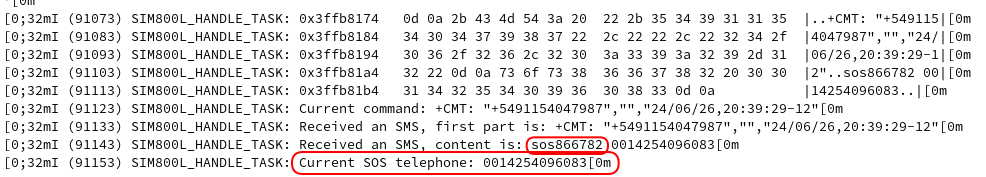
\includegraphics[width=1\textwidth]{./Figures/esp32-sos.png}
	\caption{Configuración de número telefónico para la recepción de alertas}
	\label{fig:esp32:sos}
\end{figure}


En la tabla \ref{tab:pruebas:energia} se puede observar el listado de consumo energético medido:

\begin{table}[H]
	\centering
	\caption[Tabla de consumo energético]{Tabla con mediciones de consumo energético}
	\begin{tabular}{l c c c}    
		\toprule
		\textbf{Elemento} 	 & \textbf{\makecell{Consumo \\ base}} & \textbf{\makecell{Consumo optimizado \\ según \textit{datasheet} }} & \textbf{\makecell{Consumo optimizado \\ según pruebas}}  \\
		\midrule
		ESP32-S & 30 $\sim$ 68 mA\citep{ESP32:1} & 20 mA\citep{ESP32:1} & 16 mA \\		
		LM2596 & 20 mA\citep{LM2596:1} & 5 mA &  12 mA \\	
		NEO-6M & 41 mA\citep{NEO6M:2} & 8 mA & 11 $\sim$ 30 mA \\	
		SIM800L & 60 mA\citep{SIM800L:1} & $<$ 7 mA & 10 $\sim$ 40 mA \\		
		\bottomrule
		\textbf{Total} & 140 mA & 40 mA & 49 $\sim$ 98 mA \\
		\bottomrule
		\hline
	\end{tabular}
	\label{tab:pruebas:energia}
\end{table}

Para las mediciones, no se contabilizaron pequeños componentes como LEDs y resistencias ya que su consumo total, alrededor de 1 mA, representa un porcentaje despreciable del consumo total.

Por otra parte, las mediciones son promedios, no picos de consumo debido a las limitaciones del multímetro de bajo costo utilizado. De todas maneras, se pudo validar el consumo indicado por los \textit{datasheets} de los módulos, aunque se encontraron diferencias al realizar mediciones posteriores a las optimizaciones de energía. Se obsevaron grandes diferencias entre mínimos y máximos de los módulos NEO-6M y SIM800L y esto es debido a que cuando los módulos e inicializan tienen un promedio de consumo alto, siendo estabilizado el consumo transcurrido un tiempo. Para concluir, se promedió el consumo del prototipo en 60 mA, resultando un aproximado de más de 30 horas de autonomía, en condiciones ideales y suponiendo que la batería asignada efectivamente tiene la capacidad indicada. Si bien este valor no alcanza a los objetivos iniciales, significa una duración aceptable en comparación a otros modelos de dispositivos.


El cálculo de carga de la batería se realizó mediante una aproximación lineal, siendo el voltaje medido una referencia de la carga real de la batería. Se observa en la figura \ref{fig:esp32:bateria} el valor calculado en una de las pruebas:

\begin{figure}[H]
	\centering
	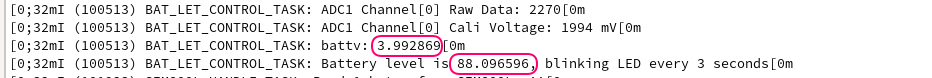
\includegraphics[width=1\textwidth]{./Figures/esp32-battery.png}
	\caption{Cálculo de carga de batería}
	\label{fig:esp32:bateria}
\end{figure}

Por último, se puede visualizar en la figura \ref{fig:esp32:alerta} el disparo de una alerta y el envío del SMS con el contenido de la localización:

\begin{figure}[H]
	\centering
	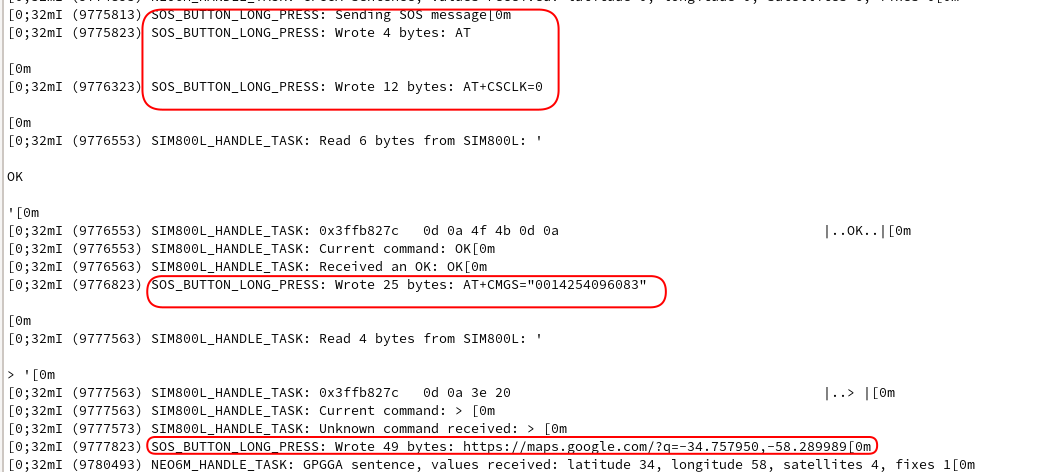
\includegraphics[width=1\textwidth]{./Figures/esp32-alerta.png}
	\caption{Disparo de alerta desde el dispositivo embebido}
	\label{fig:esp32:alerta}
\end{figure}

\subsection{Pruebas adicionales}

Debido a que se detectaron mediciones elevadas en el ESP32-S incluso aplicación de \textit{light sleep}, se realizaron pruebas adicionales con otra placa de desarrollo, ESP32-C3, cuyas prestaciones son ligeramente diferentes\citep{ESP32C3:1}. Con este dispositivo se probó solamente el firmware adaptado, sin los módulos externos, y se verificó que efectivamente el consumo era aproximadamente 1 mA. Esto permitió concluir que la placa ESP32-S de NodeMCU no está preparada para configuraciones de bajo consumo. 
De todas maneras, no se avanzó en la re-implementación del firmware debido a que implicaba acomodar varias configuraciones adicionales como el uso de puertos serie, pines en uso, entre otros. En caso de haber continuado con la implementación del modo \textit{light sleep} de forma automática, hubiera sido necesario volver a realizar pruebas con todos los módulos. La ventaja de utilizar el modo automático de \textit{light sleep} es que gran parte del tiempo \textit{idle} del ESP32 hubiera representado un ahorro de energía de varios mA.

Por otra parte, se intentó reemplazar el regulador de tensión LM2596 por el regulador de tensión lineal LD1117 cuyo consumo en es menor\citep{LD1117:1}, pero el \textit{dropout} de voltaje resultó muy elevado para el ESP32 y el NEO-6M, al punto de no ser suficiente para que funcionen correctamente.

\section{Pruebas de sistema web}

En esta sección se presentan las pruebas implementadas para los componentes del sistema web, diferenciadas por las pruebas a nivel API y las pruebas a nivel aplicación usuario.

\subsection{Pruebas de \textit{backend}}

La figura \ref{fig:tests-unitarios} muestra la ejecución correcta de los 24 tests unitarios desarrollados con la biblioteca \textit{APITestCase} de \textit{backend}:

\begin{figure}[H]
	\centering
	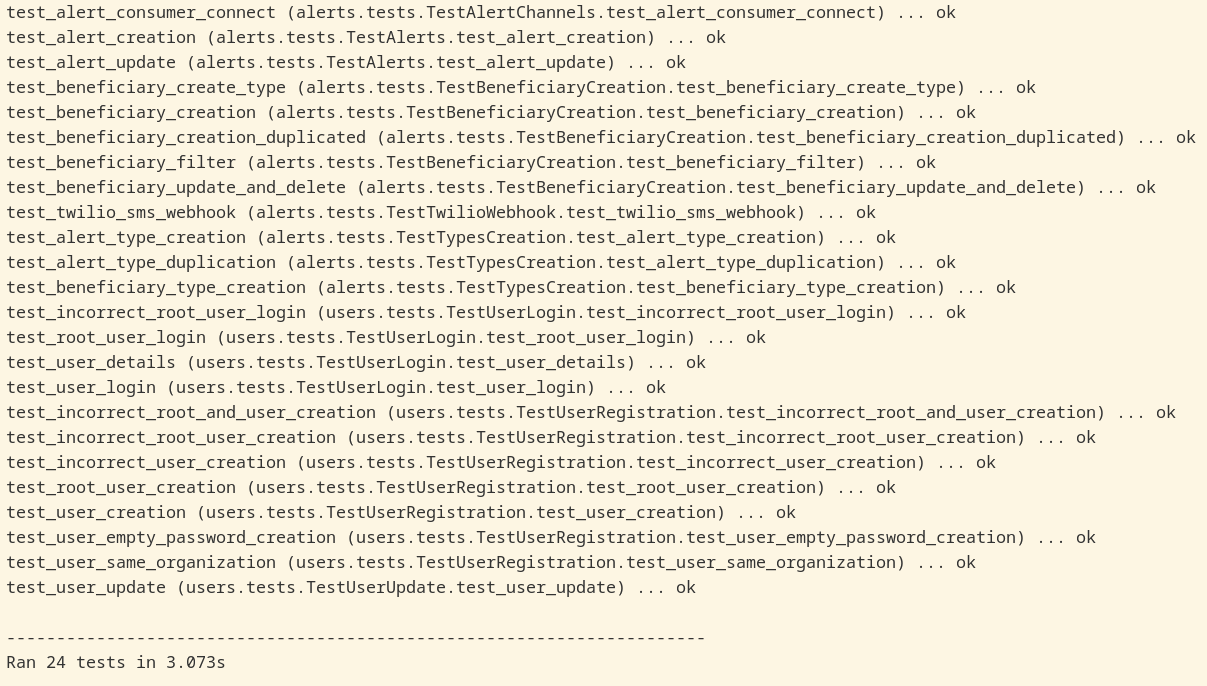
\includegraphics[width=1\textwidth]{./Figures/tests-unitarios.png}
	\caption{Ejecución correcta de tests unitarios del \textit{backend}}
	\label{fig:tests-unitarios}
\end{figure}

De todas maneras, se realizaron algunas pruebas manuales adicionales debido a casos de uso no contemplados originalmente, como actualizaciones parciales sobre entidades. Para el caso de la conexión a \textit{WebSockets}, se muestran en las figuras \ref{fig:postman1} y \ref{fig:postman2} las pruebas hechas de forma manual mediante Postman para la conexión al canal de comunicación en tiempo real y la recepción de una nueva alerta. 

\begin{figure}[H]
	\centering
  	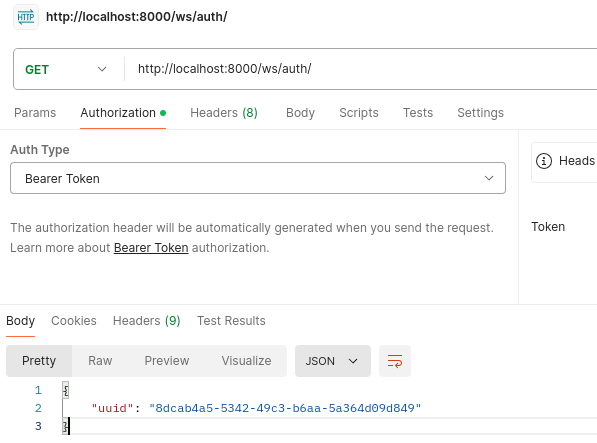
\includegraphics[width=1\linewidth]{./Figures/postman1.png}
  	\captionof{figure}{Obtención de un token efímero para \textit{WebSockets}}
  	\label{fig:postman1}
\end{figure}

En el caso de la figura \ref{fig:postman2}, se puede apreciar la marca de tiempo cuando se estableció la conexión, y más tarde se recibió publicada la nueva alerta.

\begin{figure}[H]
	\centering
  	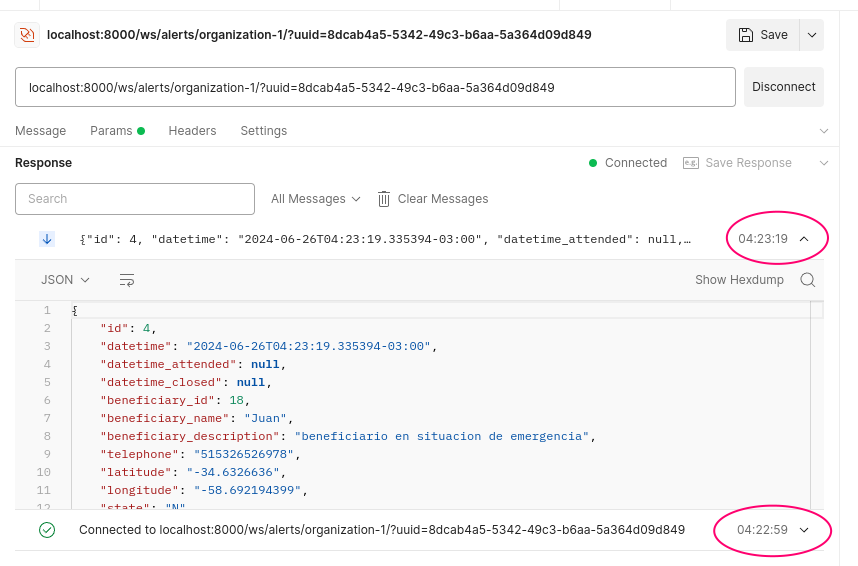
\includegraphics[width=1\linewidth]{./Figures/postman2.png}
  	\captionof{figure}{Conexión a \textit{WebSockets y recepción de una nueva alerta}}
  	\label{fig:postman2}
\end{figure}

Para la recepción de alertas de Twilio, se verificó la generación de una alerta mediante el envío de un SMS al número telefónico de Twilio. En la figura \ref{fig:backend-twilio} se puede apreciar la respuesta del \textit{backend} cuando Twilio invoca el \textit{webhook} con los datos de un número telefónico desconocido. Para probar localmente este \textit{endpoint}, se desactivó la validación de credenciales de Twilio.

\begin{figure}[H]
	\centering
  	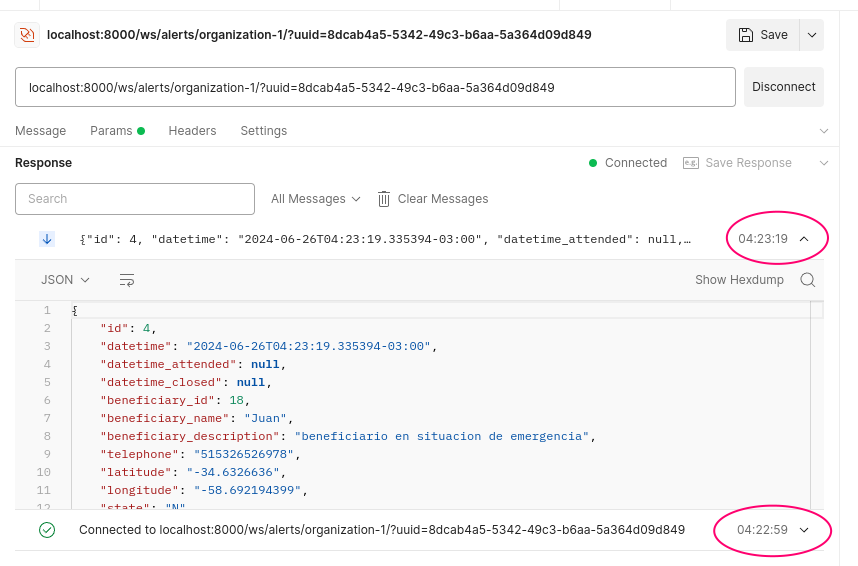
\includegraphics[width=1\linewidth]{./Figures/postman2.png}
  	\captionof{figure}{Validación de beneficiario existente al momento de generar una alerta}
  	\label{fig:backend-twilio}
\end{figure}

\subsection{Pruebas de \textit{frontend}}

Para poder verificar todos los requerimientos del \textit{frontend} listados en el banco de pruebas, se llevaron a cabo pruebas manuales sobre todas las secciones desarrolladas. En las figuras \ref{frontend:registro}, \ref{frontend:login}  se pueden apreciar las pantallas de registro y login:


\begin{figure}[H]
\centering
\begin{minipage}{.5\textwidth}
  \centering
  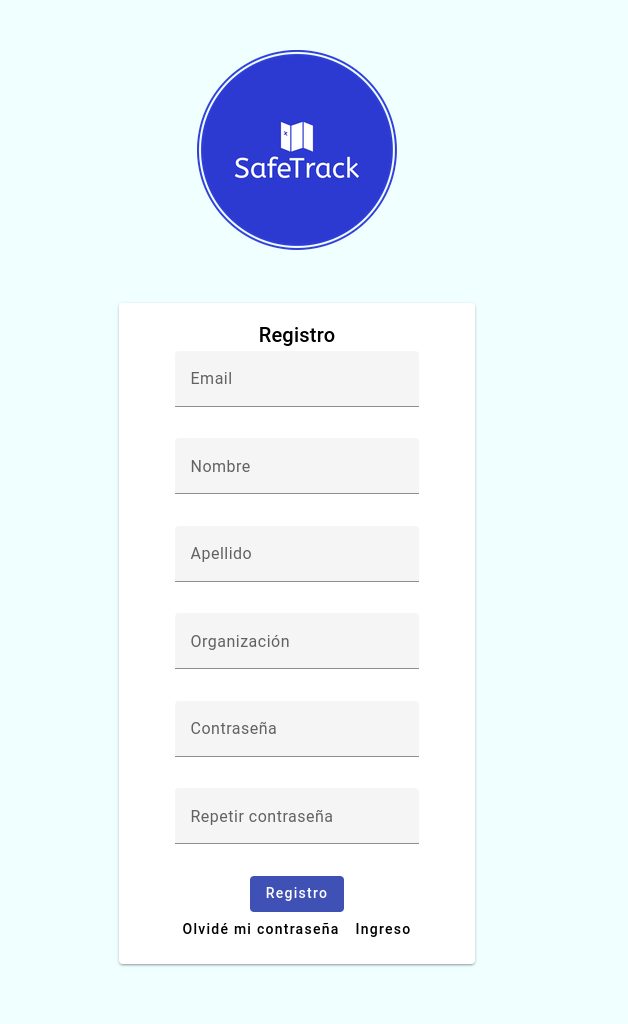
\includegraphics[width=0.9\linewidth]{./Figures/registro.png}
  \captionof{figure}{Pantalla de registro}
  \label{frontend:registro}
\end{minipage}%
\begin{minipage}{.5\textwidth}
  \centering
  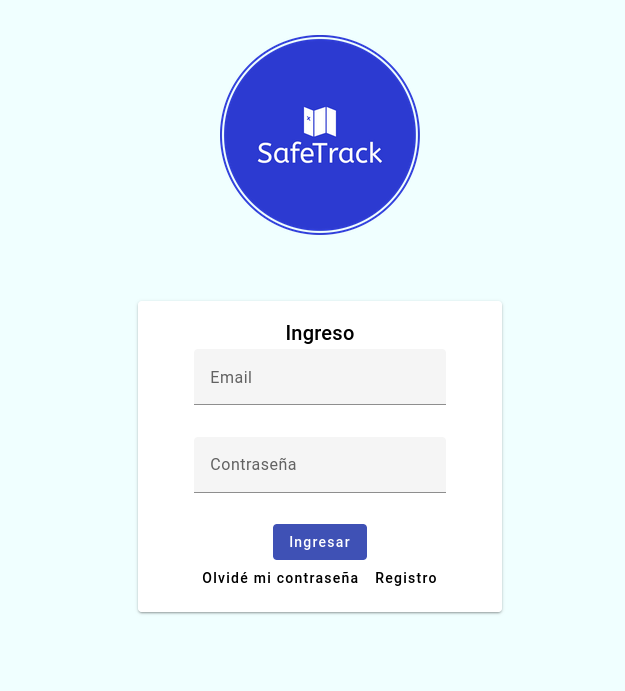
\includegraphics[width=0.9\linewidth]{./Figures/login.png}
  \captionof{figure}{Pantalla de ingreso}
  \label{frontend:login}
\end{minipage}
\end{figure}


En relación a la visualización y atención de alertas en tiempo real, se implementó la sección de mapa con el listado de alertas recientes a la izquierda, pudiendo observarse en la figura \ref{fig:frontend:mapa} una alerta generada desde el botón antipánico directamente:

\begin{figure}[H]
	\centering
  	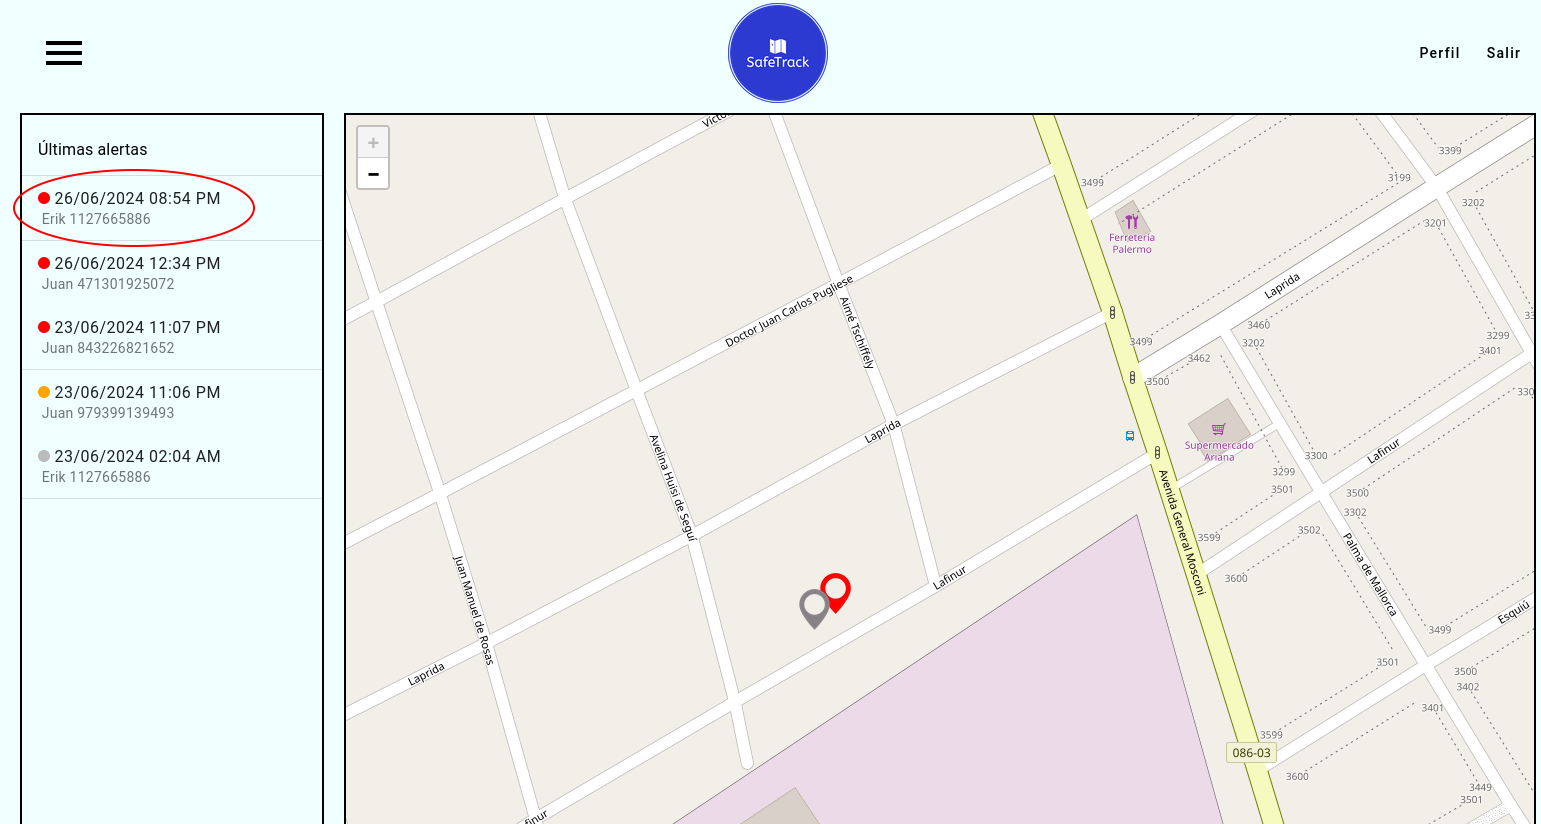
\includegraphics[width=1\linewidth]{./Figures/frontend-alerta.png}
  	\captionof{figure}{Mapa con alertas}
  	\label{fig:frontend:mapa}
\end{figure}	
	
Por otra parte se probaron los tres menús de carga creados, beneficiarios, tipos de beneficiarios y tipos de alertas, pudiendo visualizarse la sección de beneficiarios en la figura \ref{fig:frontend:beneficiarios} con algunos datos creados:

\begin{figure}[H]
	\centering
  	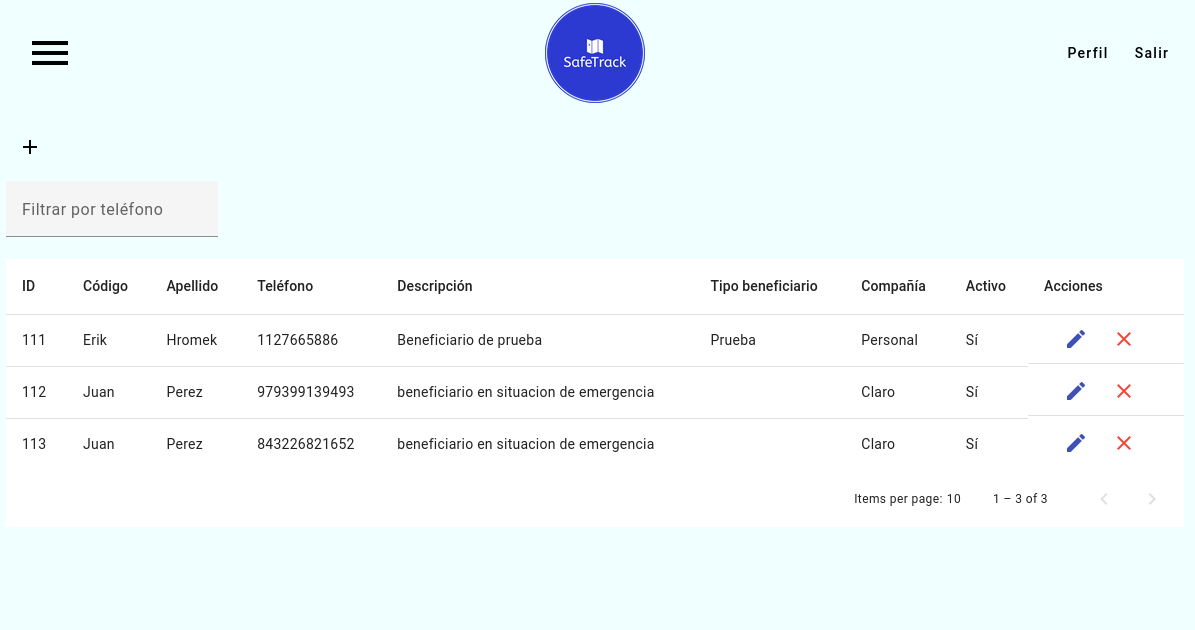
\includegraphics[width=1\linewidth]{./Figures/listado-beneficiarios.png}
  	\captionof{figure}{ABM de beneficiarios}
  	\label{fig:frontend:beneficiarios}
\end{figure}
	
Además, se implementó una sección para visualizar el historial de alertas y poder exportarlo a un archivo de extensión CSV mediante un botón, como se verifica en la figura \ref{fig:frontend:alertas}:

\begin{figure}[H]
	\centering
  	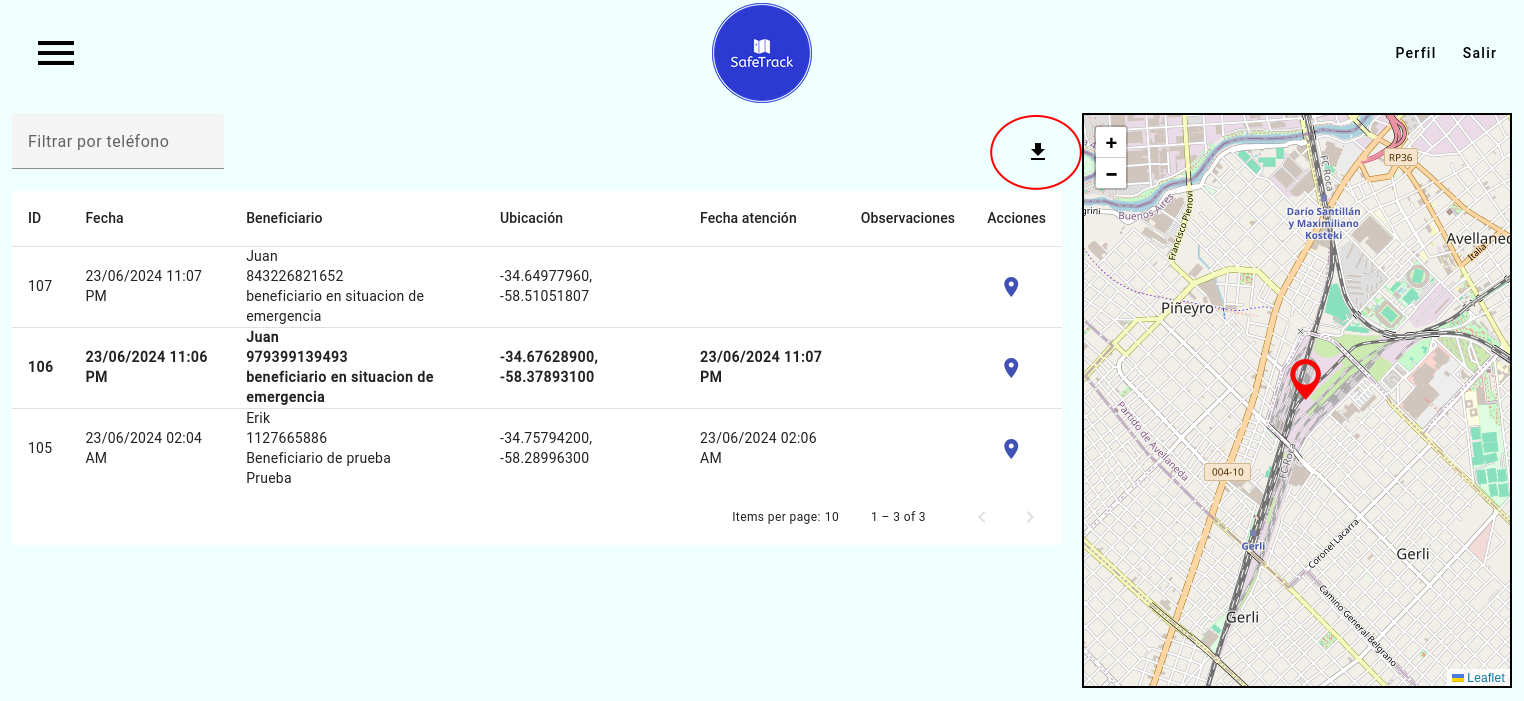
\includegraphics[width=1\linewidth]{./Figures/listado-alertas.png}
  	\captionof{figure}{Listado histórico de alertas y botón de exportación}
  	\label{fig:frontend:alertas}
\end{figure}

Todas las pruebas fueron realizadas tanto en el ambiente local de desarrollo como en el ambiente desplegado en Heroku, a excepción del envío de alertas desde Twilio debido a que fue requerido contar con una URL pública.

\section{Comparación con productos similares}

No se encuentra una solución que integre tanto el componente embebido como el sistema web de tal forma que pueda hacerse comparación uno a uno. Pero, el trabajo desarrollado permite demostrar que:
\begin{itemize}
	\item Es factible desarrollar un prototipo de botón antipánico de bajo gasto energético, si se continuara el trabajo de optimización de consumo energético de algunos componentes, como es el caso del ESP32 y el regulador LM2596.
	\item Es posible contar con un número telefónico virtual al cual se le pueden enviar las alertas por SMS y hacer que este reenviase los mensajes a otros sistemas.
	\item Se puede contar con una aplicación web básica para la recepción de alertas en tiempo real.
	\item Fue posible desarrollar un dispositivo de hardware con costos relativamente bajos, y prestaciones superiores en 
\end{itemize}

La tabla \ref{tab:comparativa} presenta una breve comparativa de puntos interesantes del dispositivo embebido contrastado contra los dos modelos de botón antipánico presentados en el capítulo 1 del documento:

\begin{table}[H]
	\centering
	\caption[Tabla comparativa de dispositivos]{Comparativa de dispositivos embebidos}
	\begin{tabular}{l c c c c}    
		\toprule
		\textbf{Modelo} & \textbf{\makecell{Duración \\ de batería}} & \textbf{\makecell{Tiempo para \\ conexión GSM}} & \textbf{\makecell{Tiempo para \\ conexión GPS}} & \textbf{\makecell{Precisión \\ GPS \textit{indoor}}} \\
		\midrule
		TK102 & Buena & Buena & Media & Media \\ 
		LK109 & Baja & Buena & Muy Buena & Media \\
		\makecell[l]{Desarrollo \\ propio} & Media & Baja & Baja & Muy buena \\		
		\bottomrule
		\hline
	\end{tabular}
	\label{tab:comparativa}
\end{table}

En relación a las capacidades de las antenas, se observó una mejoría respecto a otros modelos existentes. Respecto a la duración de la batería, se concluye que también podría ser mejorable con baterías de mayor capacidad, aunque esto implicaría un aumento en el costo del dispositivo.


 
	% Chapter Template

\chapter{Conclusiones} % Main chapter title

\label{Chapter5} % Change X to a consecutive number; for referencing this chapter elsewhere, use \ref{ChapterX}

En este capítulo se presentan las conclusiones del trabajo realizado, así como también propuestas de continuidad para el futuro.
%----------------------------------------------------------------------------------------

%----------------------------------------------------------------------------------------
%	SECTION 1
%----------------------------------------------------------------------------------------

\section{Conclusiones y resultados obtenidos}

En este trabajo se ha culminado el desarrollo y las pruebas funcionales de un prototipo de botón antipánico y un sistema web para poder recibir y gestionar las alertas recibidas.

En relación a los objetivos planteados se considera que el único objetivo que no se alcanzó fue el de poder reducir drásticamente el consumo energético de tal forma que el dispositivo pueda durar varios días, y el hecho de querer plantear el desarrollo embebido como un proyecto que sea rápidamente extensible, como una biblioteca. Por otra parte, los demás objetivos sí se pudieron cumplir, y se considera importante destacarlo, para evidenciar el valor y aporte del desarrollo del trabajo. Debido a esto, se orientó la etapa final del desarrollo a poder completar de una forma más abarcativa los demás componentes involucrados para que puedan aprovecharse para proyectos futuros.

En base a las conclusiones y resultados generales, se puede analizar el grado de cumplimiento de todos los requerimientos en el anexo \ref{AppendixA}. Se observa que la mayor cantidad de inconvenientes estuvo relacionada con las dificultades para cumplir con la optimización del consumo energético.

En relación a los objetivos no cumplidos, se debe al hecho de haber subestimado el trabajo a realizar sobre el sistema embebido y la poca experiencia en el desarrollo de sistemas embebidos de este tipo. Otro factor que influyó fue la dificultad para realizar pruebas exhaustivas sobre los componentes de hardware.

Se considera que la planificación original fue acorde al tiempo requerido, a excepción del módulo embebido cuya complejidad e inconvenientes detectados fueron considerables. Respecto a la organización del tiempo, se presentaron imprevistos laborales que obligaron a posponer la finalización del desarrollo.

A pesar de los desafíos atravesados y teniendo en cuenta tanto los entregables como los resultados, se considera que el resultado del trabajo fue muy positivo, destacando el aprendizaje, la experiencia adquirida y el desarrollo de un prototipo con la posibilidad de continuar el trabajo.

%----------------------------------------------------------------------------------------
%	SECTION 2
%----------------------------------------------------------------------------------------
\section{Trabajo futuro}

En relación al trabajo futuro, se pueden tener en cuenta dos aristas para aprovechar el trabajo realizado y extenderlo hacia el futuro. A continuación, se detallan los principales puntos que se pueden desarrollar y trabajar hacia adelante.

\begin{itemize}
	\item Tomar como referencia todo lo aplicado para el desarrollo con el framework ESP-IDF, y lo que se investigó pero no se pudo aplicar correctamente e implementarlo para otras placas similares, que tengan algunas características de hardware resueltas o ya incorporadas. Este el caso de la placa de desarrollo \textit{LilyGo SIM7000G}, que integra módulos de telefonía móvil, GPS, batería, etc. en un mismo kit \citep{7600G:1}. Además, incluye la posibilidad de utilizar redes de bajo consumo como NB-IoT \citep{NBIOT:1} ya que posee un módulo GSM más moderno que el utilizado en el trabajo.
	\item Convertir el \textit{Minimun Viable Product} o MVP del sistema web en un producto final o incorporar las funcionalidades consideradas más útiles en un producto \textit{legacy} del empleo actual del autor con características muy similares, como es la parte de \textit{WebSockets}, API REST e integración con números telefónicos virtuales.
	\item Extender la funcionalidad del \textit{frontend} para contemplar múltiples usuarios de una misma organización o ambiente, teniendo ya la implementación en la API.
	\item Incorporar una estructura del \textit{layout} de la aplicación web que sea adaptable a dispositivos móviles.
	\item Incorporar la posibilidad de recibir alertas no solamente mediante SMS, sino también mediante otras aplicaciones como \textit{Whatsapp}, cuya integración puede hacerse vía APIs \citep{TWILIO:3}.
	\item Agregar de funcionalidades de seguimiento continuo en el sistema embebido para vehículos, sabiendo que hay trabajos realizados sobre el tema, pero considerando incorporar alimentación de energía continua.
\end{itemize}
 
\end{verbatim}

Los apéndices también deben escribirse en archivos .tex separados, que se deben ubicar dentro de la carpeta \emph{Appendices}. Los apéndices vienen comentados por defecto con el caracter \code{\%} y para incluirlos simplemente se debe eliminar dicho caracter.

Finalmente, se encuentra el código para incluir la bibliografía en el documento final.  Este código tampoco debe modificarse. La metodología para trabajar las referencias bibliográficas se desarrolla en la sección \ref{sec:biblio}.
%----------------------------------------------------------------------------------------

\section{Bibliografía}
\label{sec:biblio}

Las opciones de formato de la bibliografía se controlan a través del paquete de latex \option{biblatex} que se incluye en la memoria en el archivo memoria.tex.  Estas opciones determinan cómo se generan las citas bibliográficas en el cuerpo del documento y cómo se genera la bibliografía al final de la memoria.

En el preámbulo se puede encontrar el código que incluye el paquete biblatex, que no requiere ninguna modificación del usuario de la plantilla, y que contiene las siguientes opciones:

\begin{lstlisting}
\usepackage[backend=bibtex,
	natbib=true, 
	style=numeric, 
	sorting=none]
{biblatex}
\end{lstlisting}

En el archivo \file{reference.bib} se encuentran las referencias bibliográficas que se pueden citar en el documento.  Para incorporar una nueva cita al documento lo primero es agregarla en este archivo con todos los campos necesario.  Todas las entradas bibliográficas comienzan con $@$ y una palabra que define el formato de la entrada.  Para cada formato existen campos obligatorios que deben completarse. No importa el orden en que las entradas estén definidas en el archivo .bib.  Tampoco es importante el orden en que estén definidos los campos de una entrada bibliográfica. A continuación se muestran algunos ejemplos:

\begin{lstlisting}
@ARTICLE{ARTICLE:1,
    AUTHOR="John Doe",
    TITLE="Title",
    JOURNAL="Journal",
    YEAR="2017",
}
\end{lstlisting}


\begin{lstlisting}
@BOOK{BOOK:1,
    AUTHOR="John Doe",
    TITLE="The Book without Title",
    PUBLISHER="Dummy Publisher",
    YEAR="2100",
}
\end{lstlisting}


\begin{lstlisting}
@INBOOK{BOOK:2,
    AUTHOR="John Doe",
    TITLE="The Book without Title",
    PUBLISHER="Dummy Publisher",
    YEAR="2100",
    PAGES="100-200",
}
\end{lstlisting}




Se debe notar que los nombres \emph{ARTICLE:1}, \emph{BOOK:1}, \emph{BOOK:2} y \emph{WEBSITE:1} son nombres de fantasía que le sirve al autor del documento para identificar la entrada. En este sentido, se podrían reemplazar por cualquier otro nombre.  Tampoco es necesario poner : seguido de un número, en los ejemplos sólo se incluye como un posible estilo para identificar las entradas.

La entradas se citan en el documento con el comando: 

\begin{verbatim}
\citep{nombre_de_la_entrada}
\end{verbatim}

Y cuando se usan, se muestran así: \citep{ARTICLE:1}, \citep{BOOK:1}, \citep{BOOK:2}, \citep{WEBSITE:1}.  Notar cómo se conforma la sección Bibliografía al final del documento.

Finalmente y como se mencionó en la subsección \ref{subsec:configurando}, para actualizar las referencias bibliográficas tanto en la sección bibliografía como las citas en el cuerpo del documento, se deben ejecutar las herramientas de compilación PDFLaTeX, BibTeX, PDFLaTeX, PDFLaTeX, en ese orden.  Este procedimiento debería resolver cualquier mensaje "Citation xxxxx on page x undefined".
